\documentclass[cn,pad,chinese,chinesefont=nofont]{elegantbook}
\usepackage{latexgit}
\usepackage{hyperref}
\usepackage{hyperxmp}
\hypersetup{
	pdftitle={Dongxiao Mannual},
    pdfauthor={xue35},
    pdfcopyright={Copyright (C) 2020 by Jianmin Xue.  All rights reserved.}
}
%\usepackage{showframe}
\setCJKmainfont{Source Han Serif} 
\setCJKsansfont{Source Han Sans} 
\setCJKmonofont{Source Han Mono} 
\setCJKfamilyfont{zhsong}{Source Han Serif}
\setCJKfamilyfont{zhhei}{Source Han Sans} 
\setCJKfamilyfont{zhkai}{Source Han Mono} 
\setCJKfamilyfont{zhfs}{Source Han Mono} 
\newcommand*{\songti}{\CJKfamily{zhsong}} 
\newcommand*{\heiti}{\CJKfamily{zhhei}} 
\newcommand*{\kaishu}{\CJKfamily{zhkai}} 
\newcommand*{\fangsong}{\CJKfamily{zhfs}}

\title{洞箫演奏入门 - 筒音5}
\author{雪散舞}
\date{\zhtoday}
\cover{dongxiao/cover.jpeg}
\logo{monk.png}
\extrainfo{清籁远喑喑,秦楼夜思深。碧空人已去,沧海凤难寻。\\杳妙和云绝,依微向水沉。还将九成意,高阁伫芳音。}
\version{\gitcommithash}

\begin{document}
\maketitle
\frontmatter
\tableofcontents
\mainmatter

\centering
\chapter{筒音做‘低音5’}
\section{指法表}
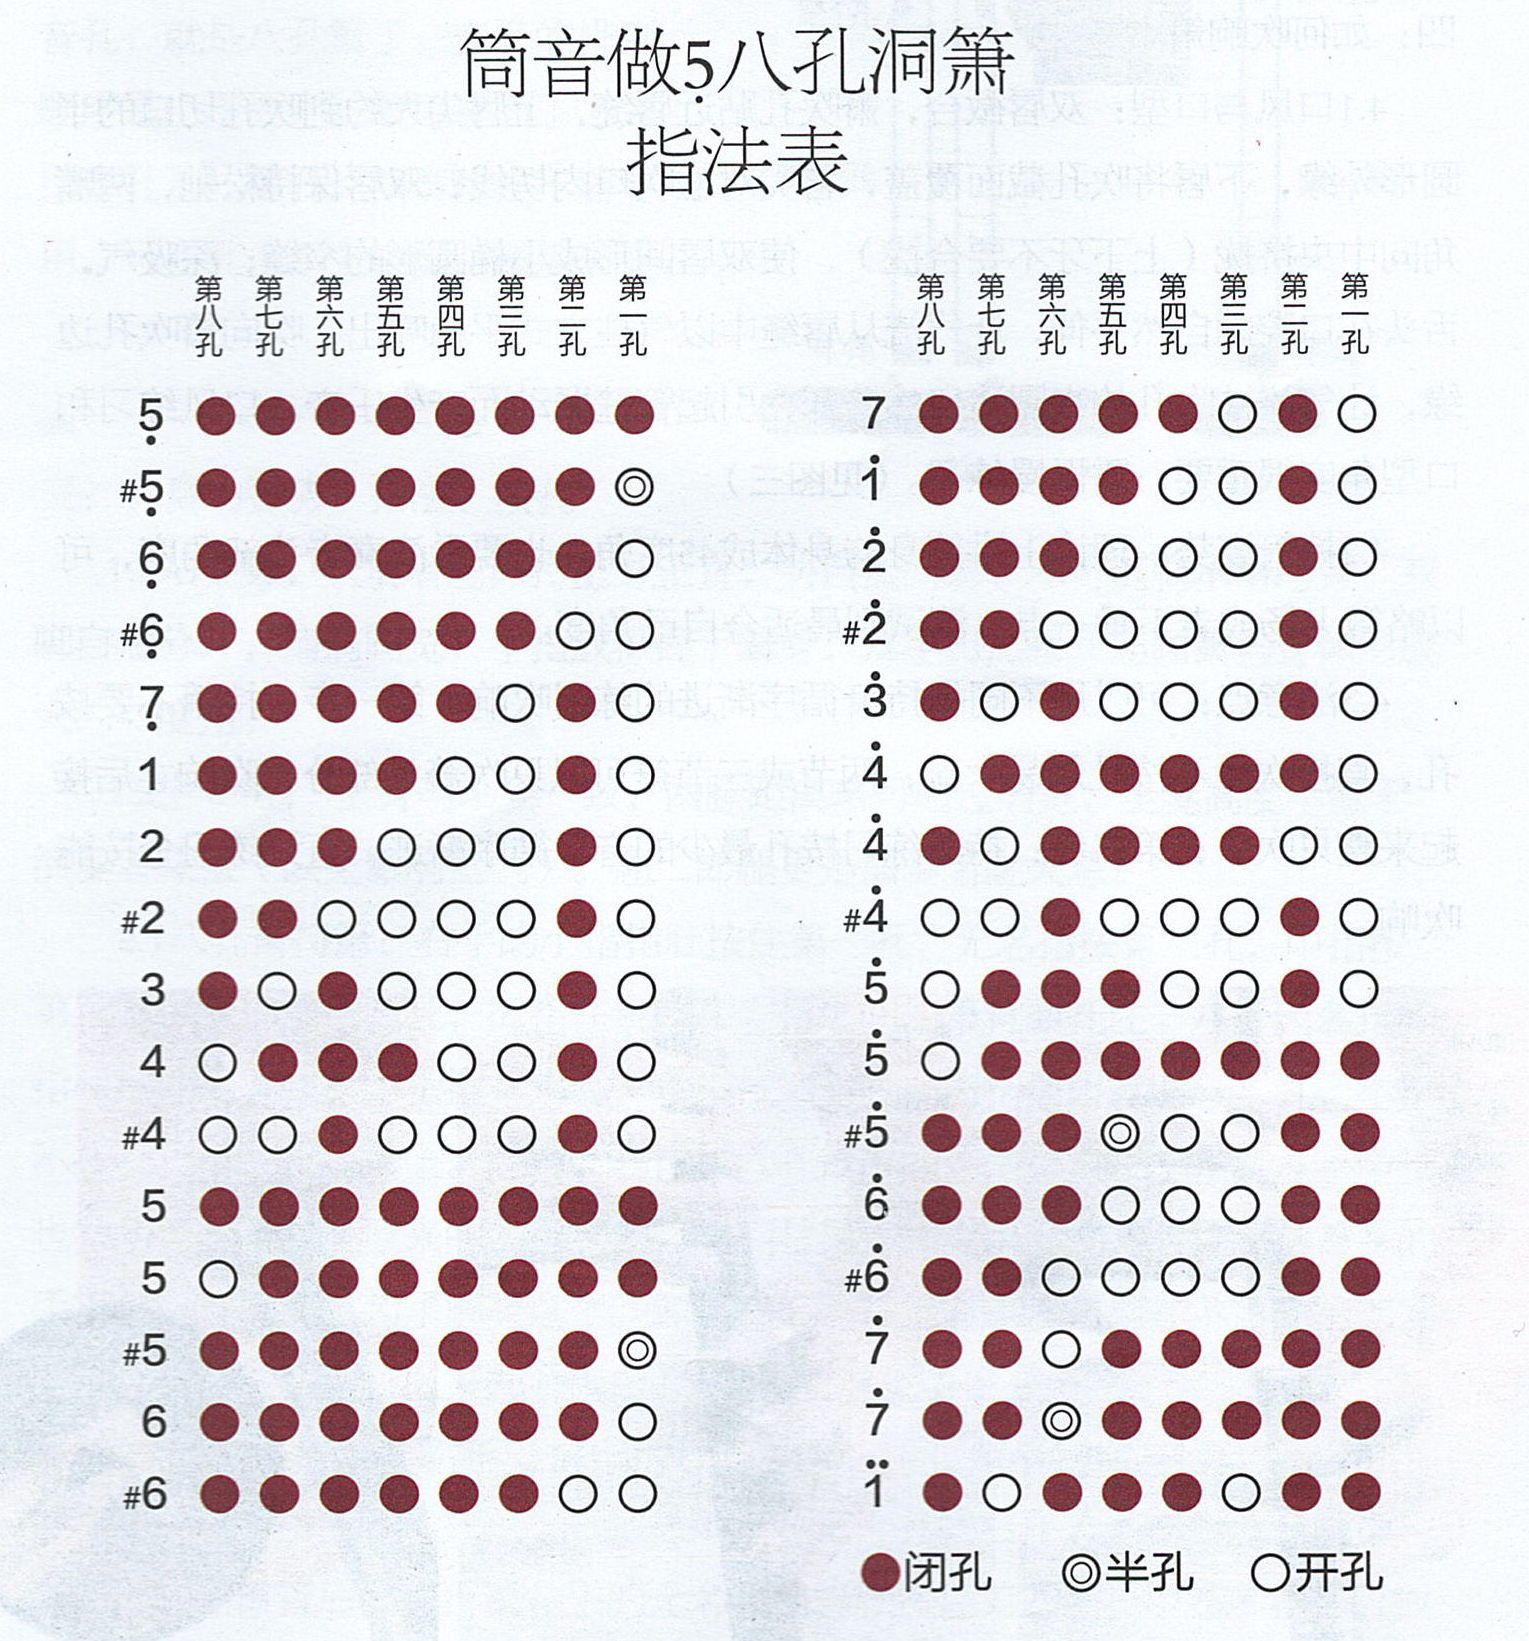
\includegraphics[width=\textwidth]{dongxiao/Scan.jpeg}

\section{内蒙民歌}
	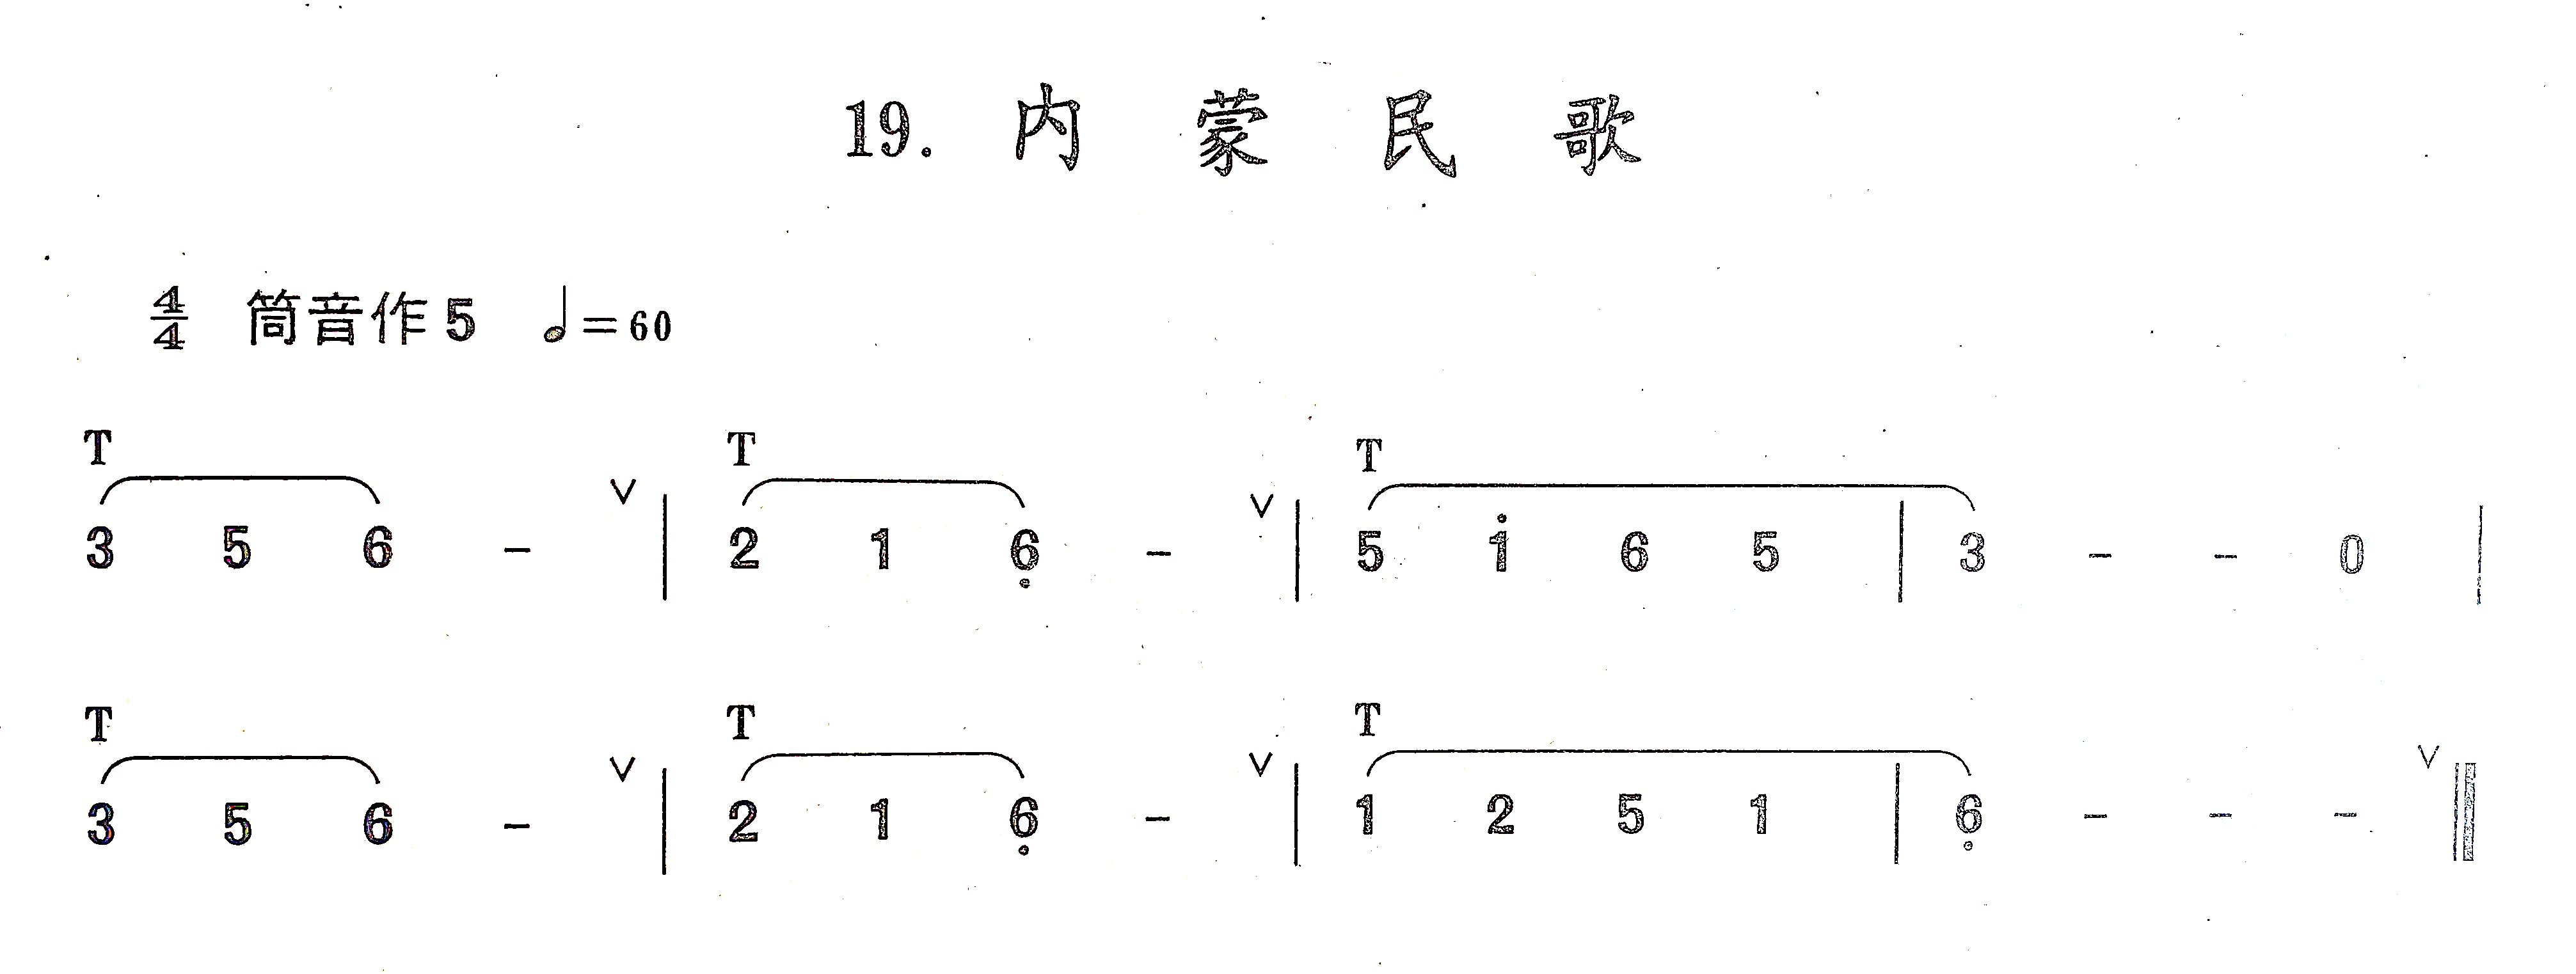
\includegraphics[width=\textwidth]{dongxiao/IMG0944内蒙民歌.jpg}  
\section{世上只有妈妈好}
	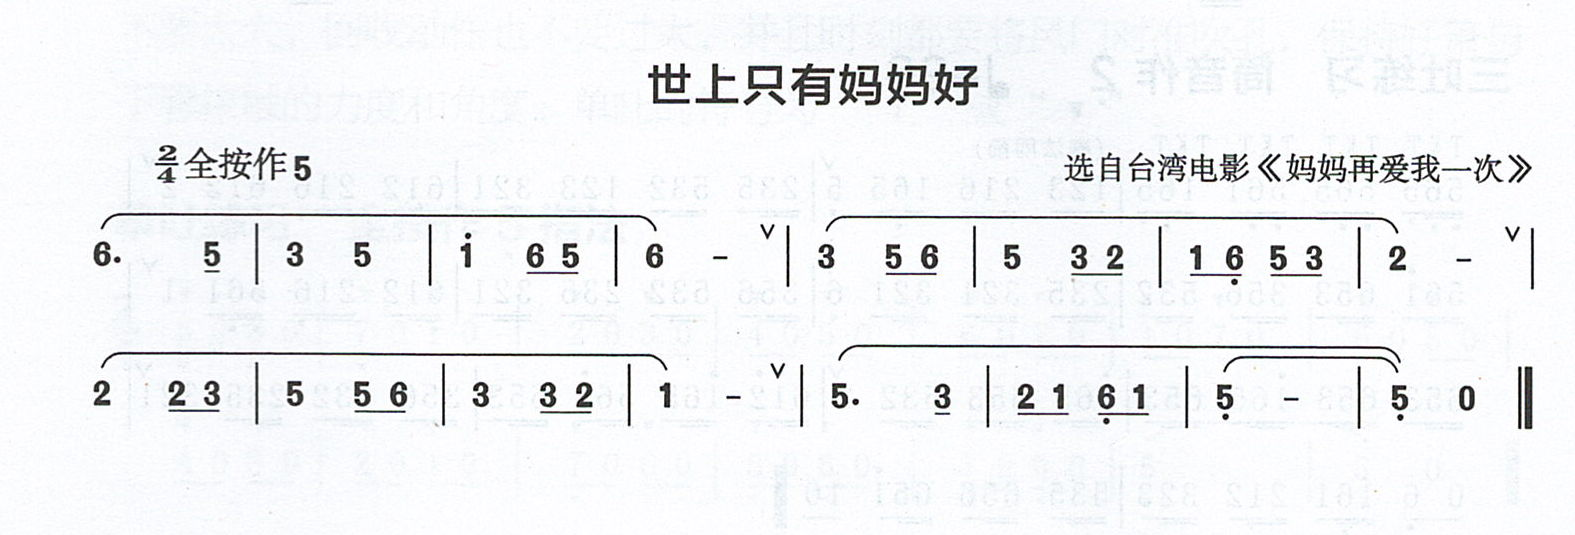
\includegraphics[width=\textwidth]{dongxiao/Scan 17-1.jpeg}
\section{送别}
    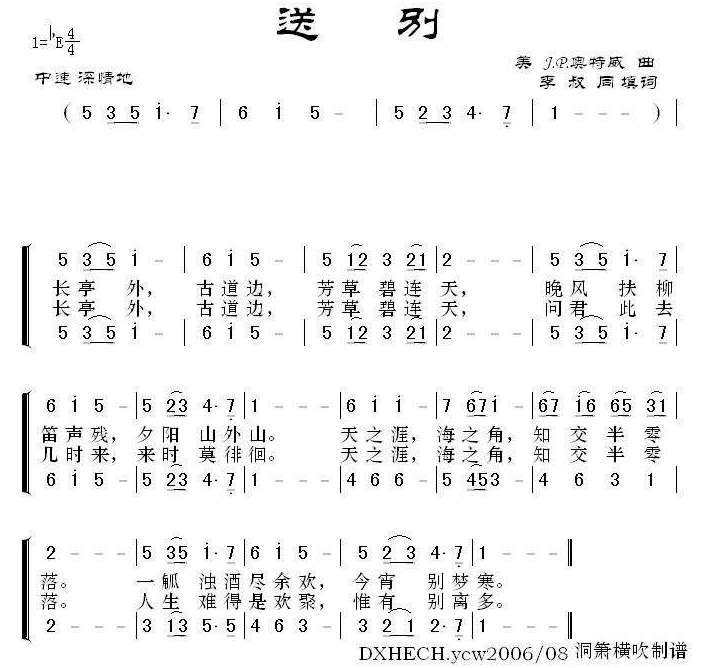
\includegraphics[width=\textwidth]{dongxiao/20200324送别.jpg}  
\section{小白菜}            
	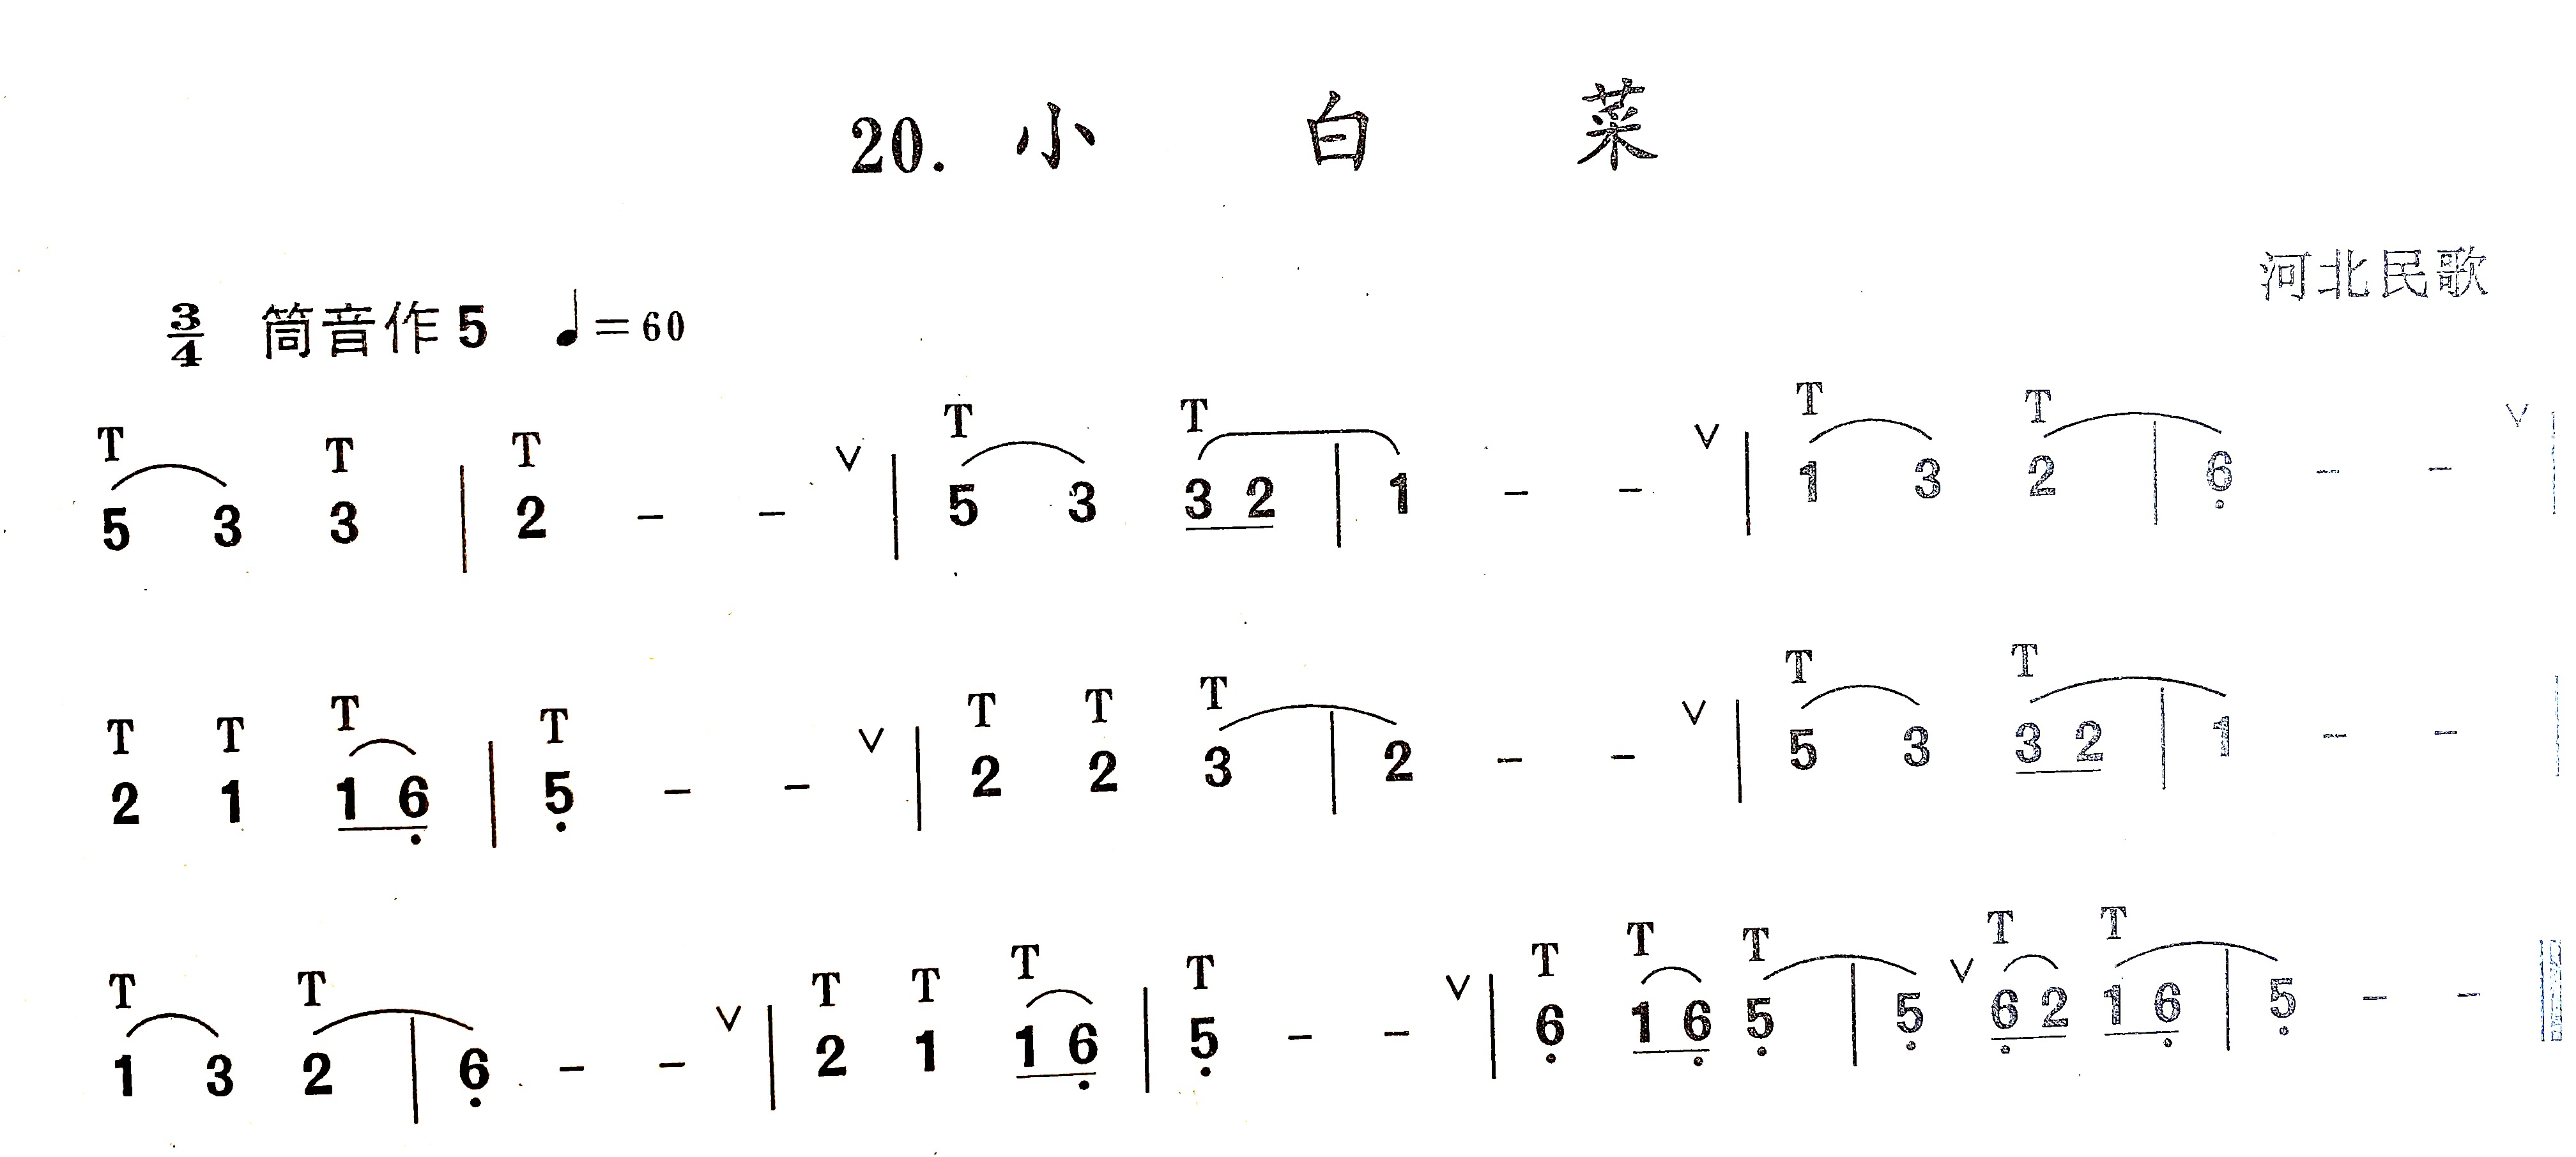
\includegraphics[width=\textwidth]{dongxiao/IMG_0933.jpg}                  
\section{长城谣}
	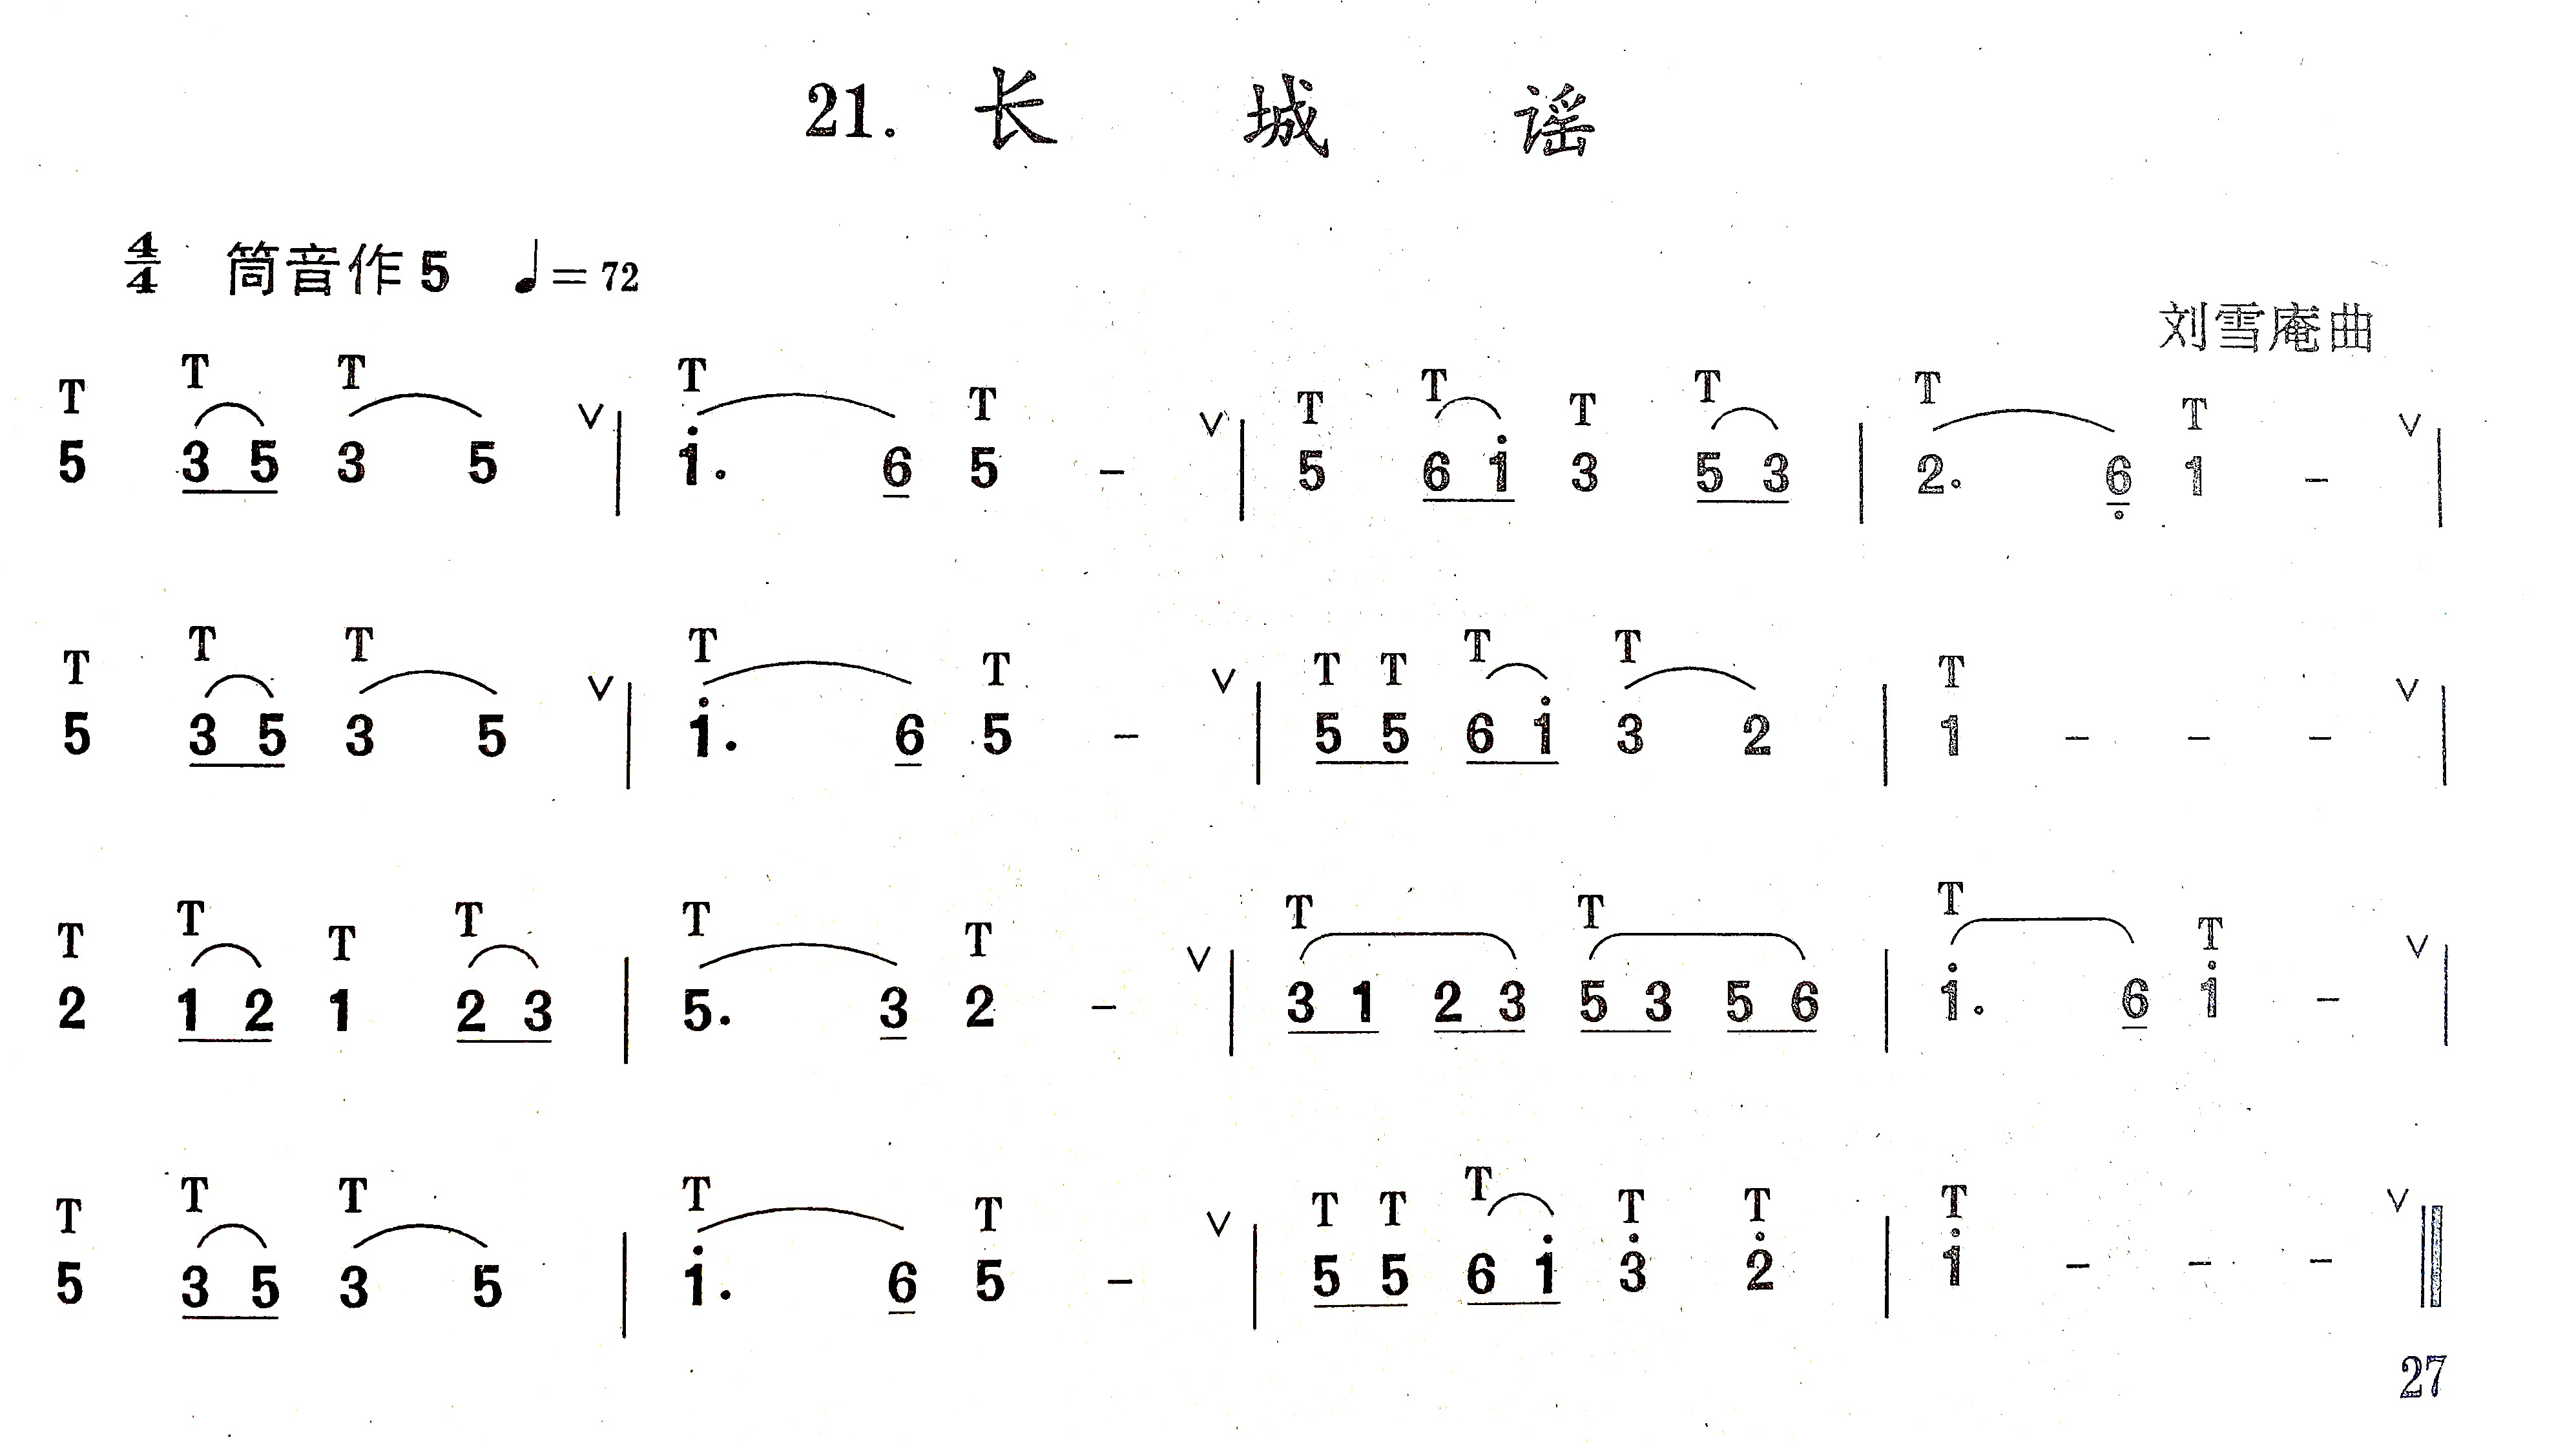
\includegraphics[width=\textwidth]{dongxiao/IMG_0934.jpg} 
\section{苏武牧羊}
	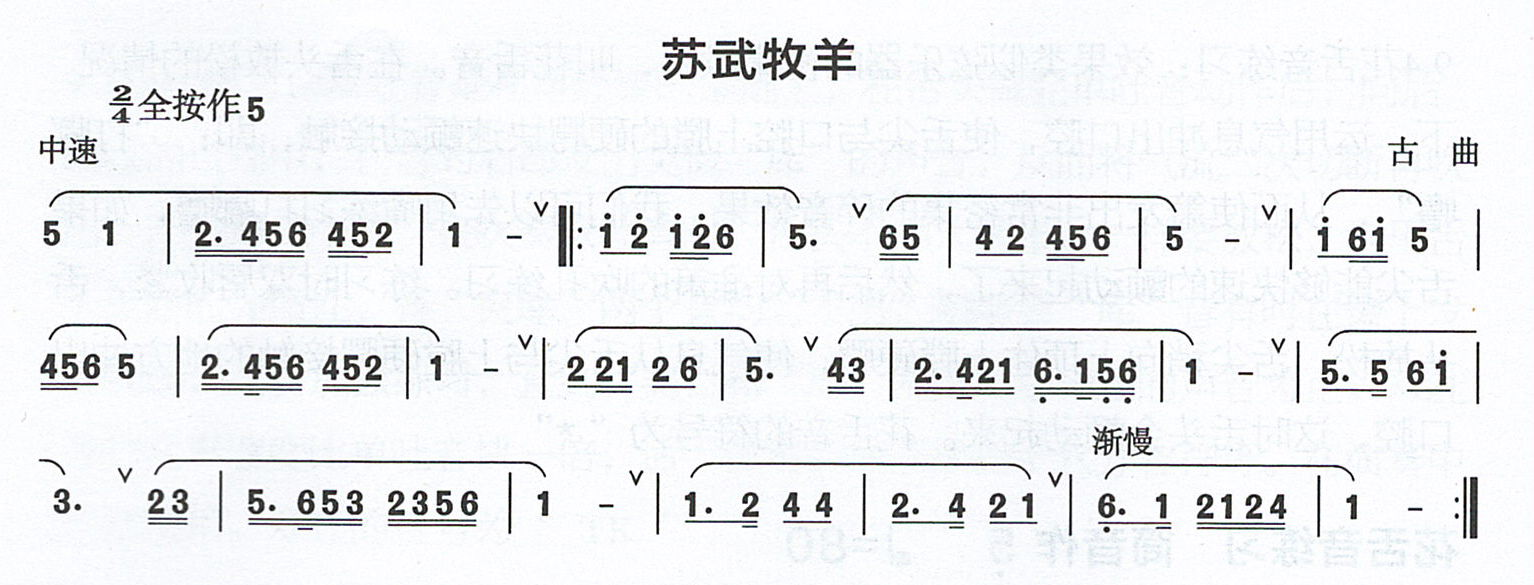
\includegraphics[width=\textwidth]{dongxiao/Scan 17-2.jpeg}
\section{嘎达梅林}
	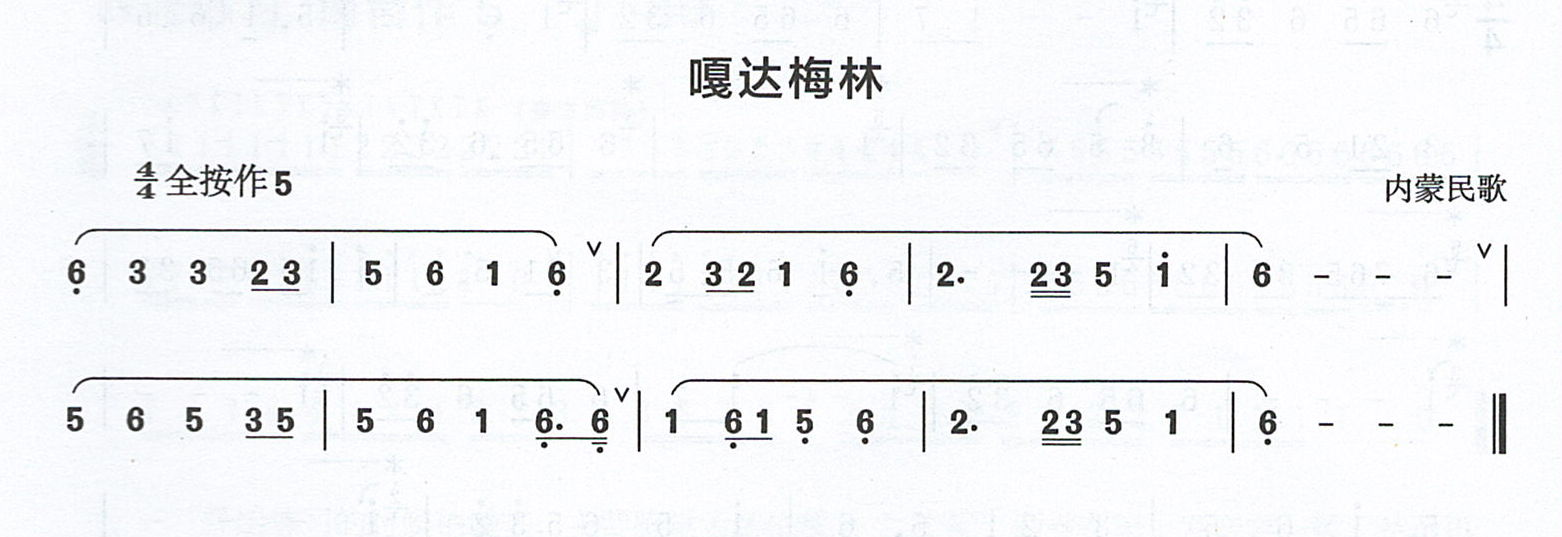
\includegraphics[width=\textwidth]{dongxiao/Scan 17-3.jpeg}
      
\section{西湖春}          
	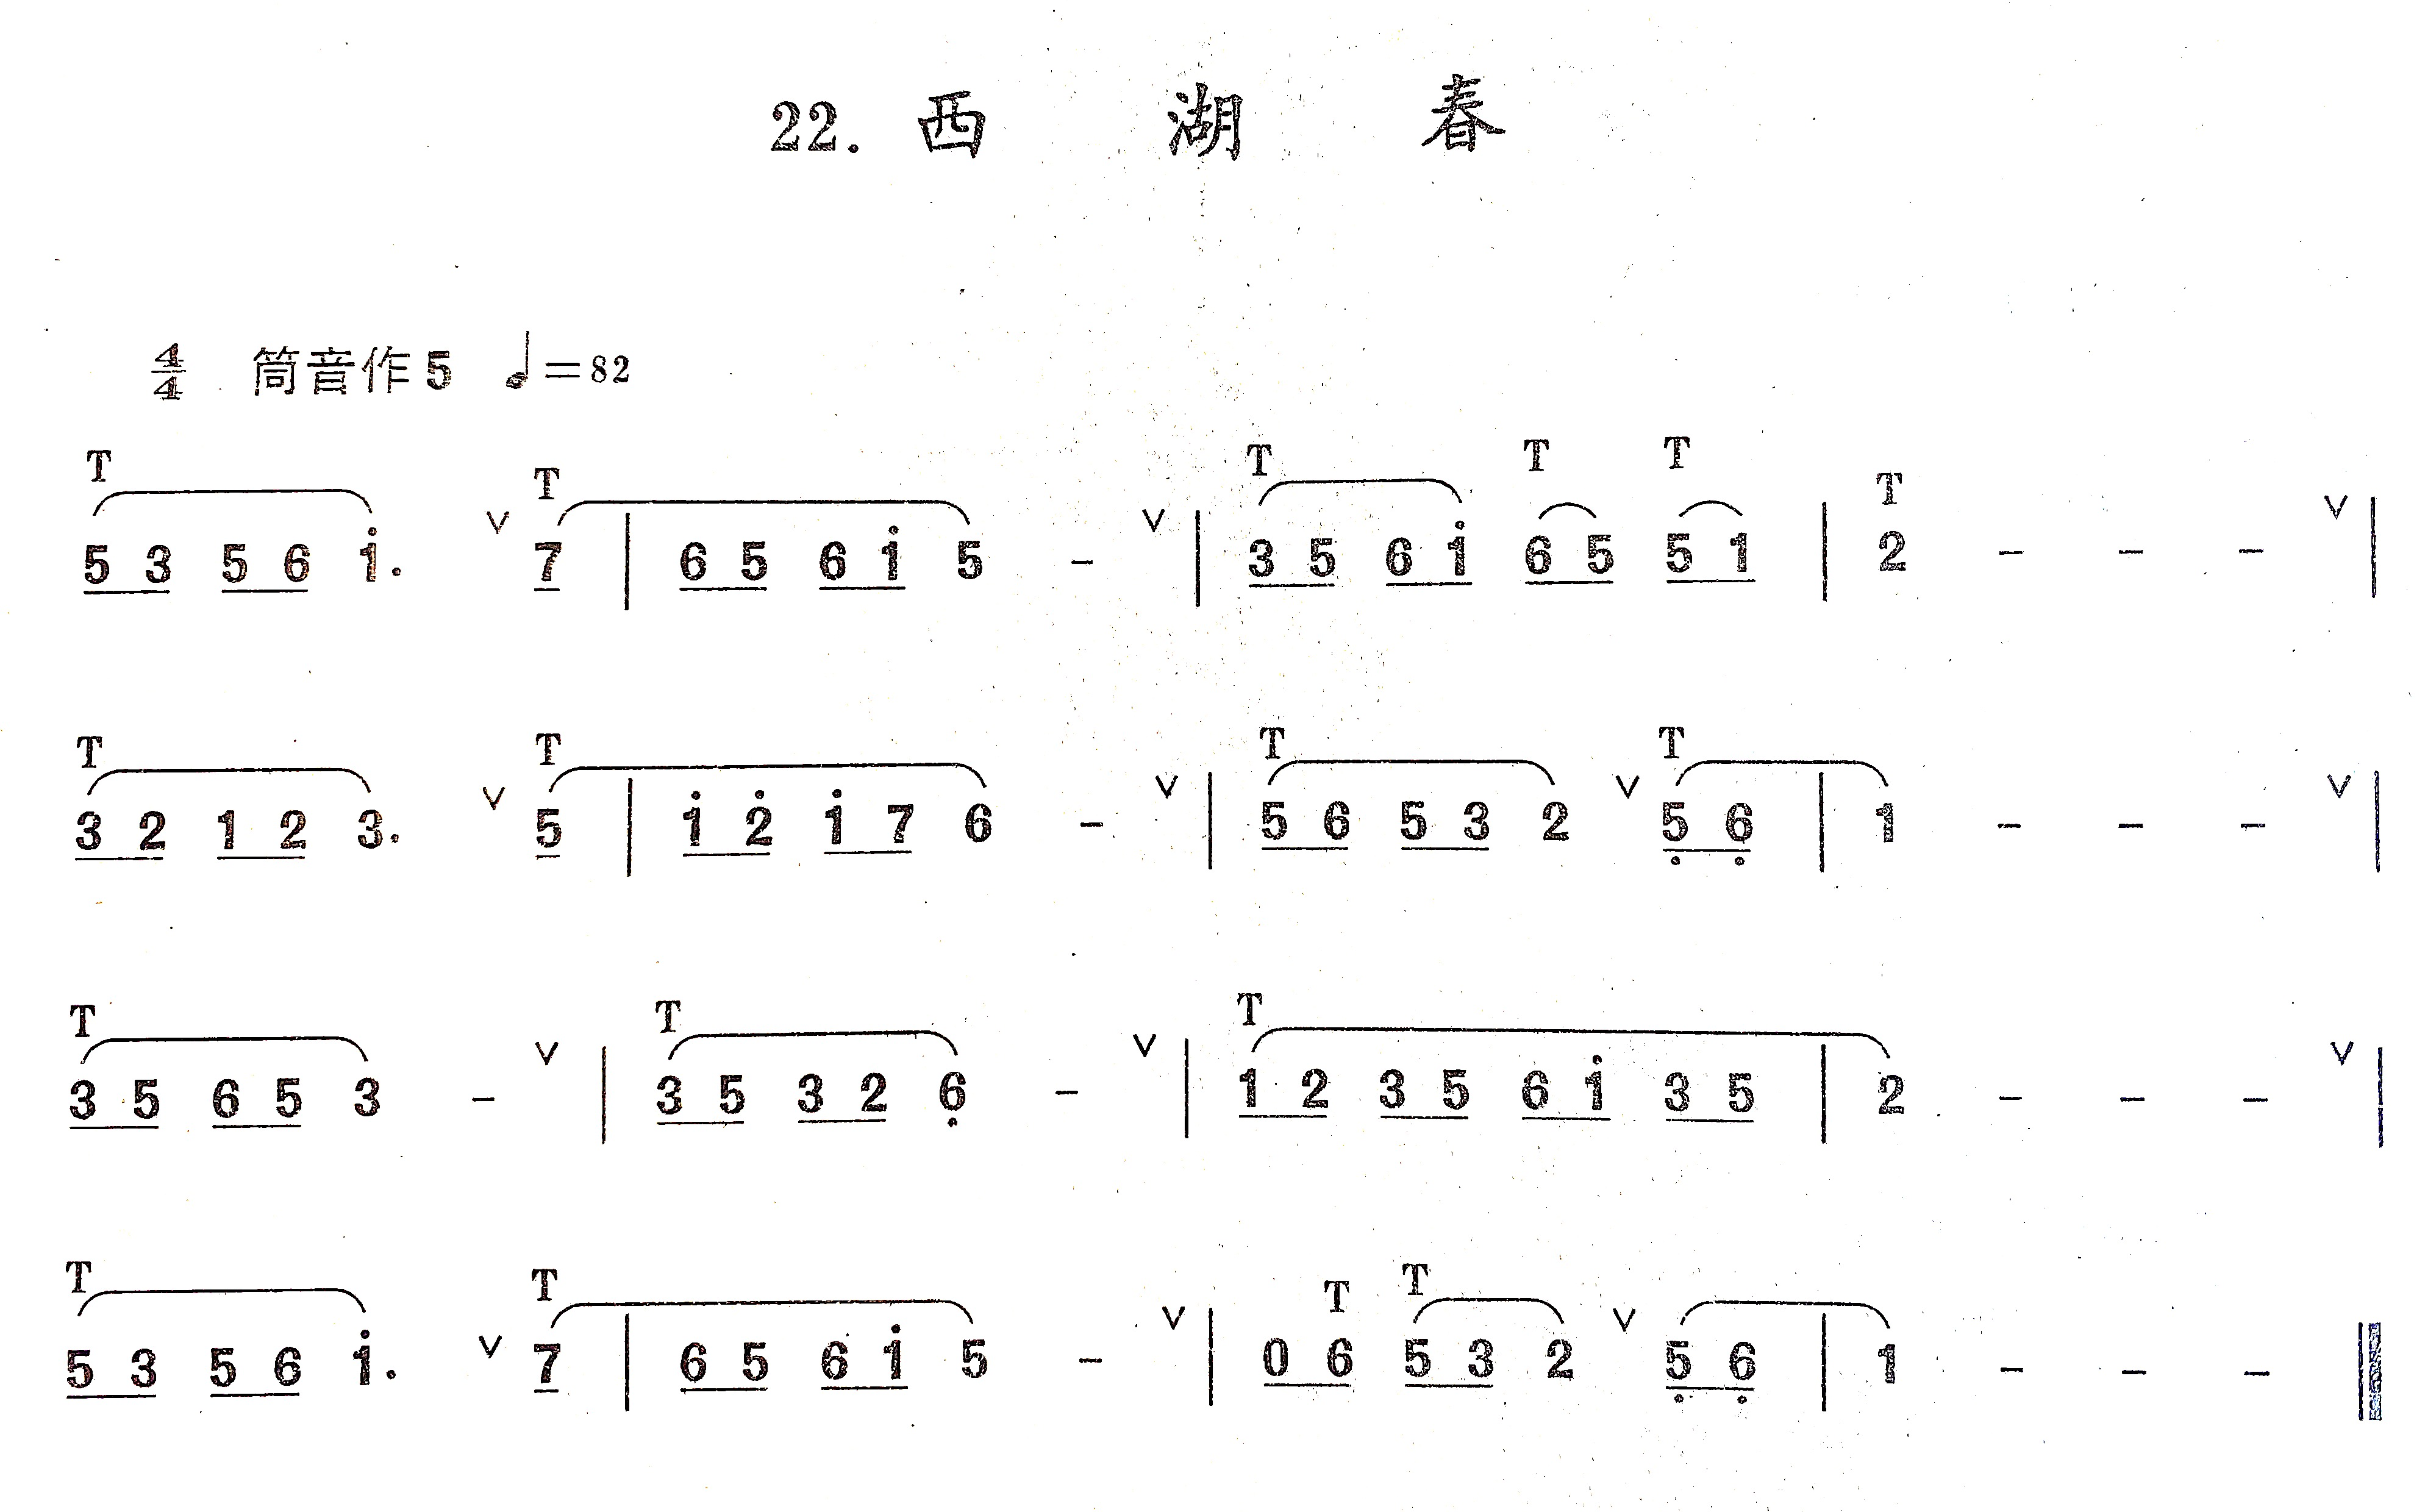
\includegraphics[width=\textwidth]{dongxiao/IMG_0935.jpg} 
\section{闹莲花}
    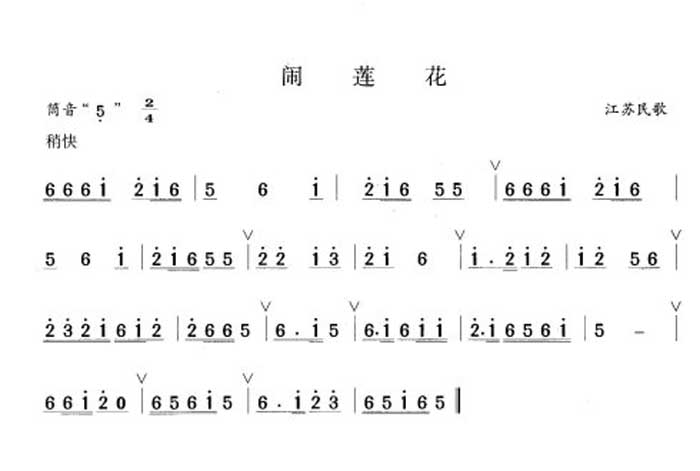
\includegraphics[width=\textwidth]{dongxiao/20200323凄凉犯.jpg}    
\section{补破网}           
	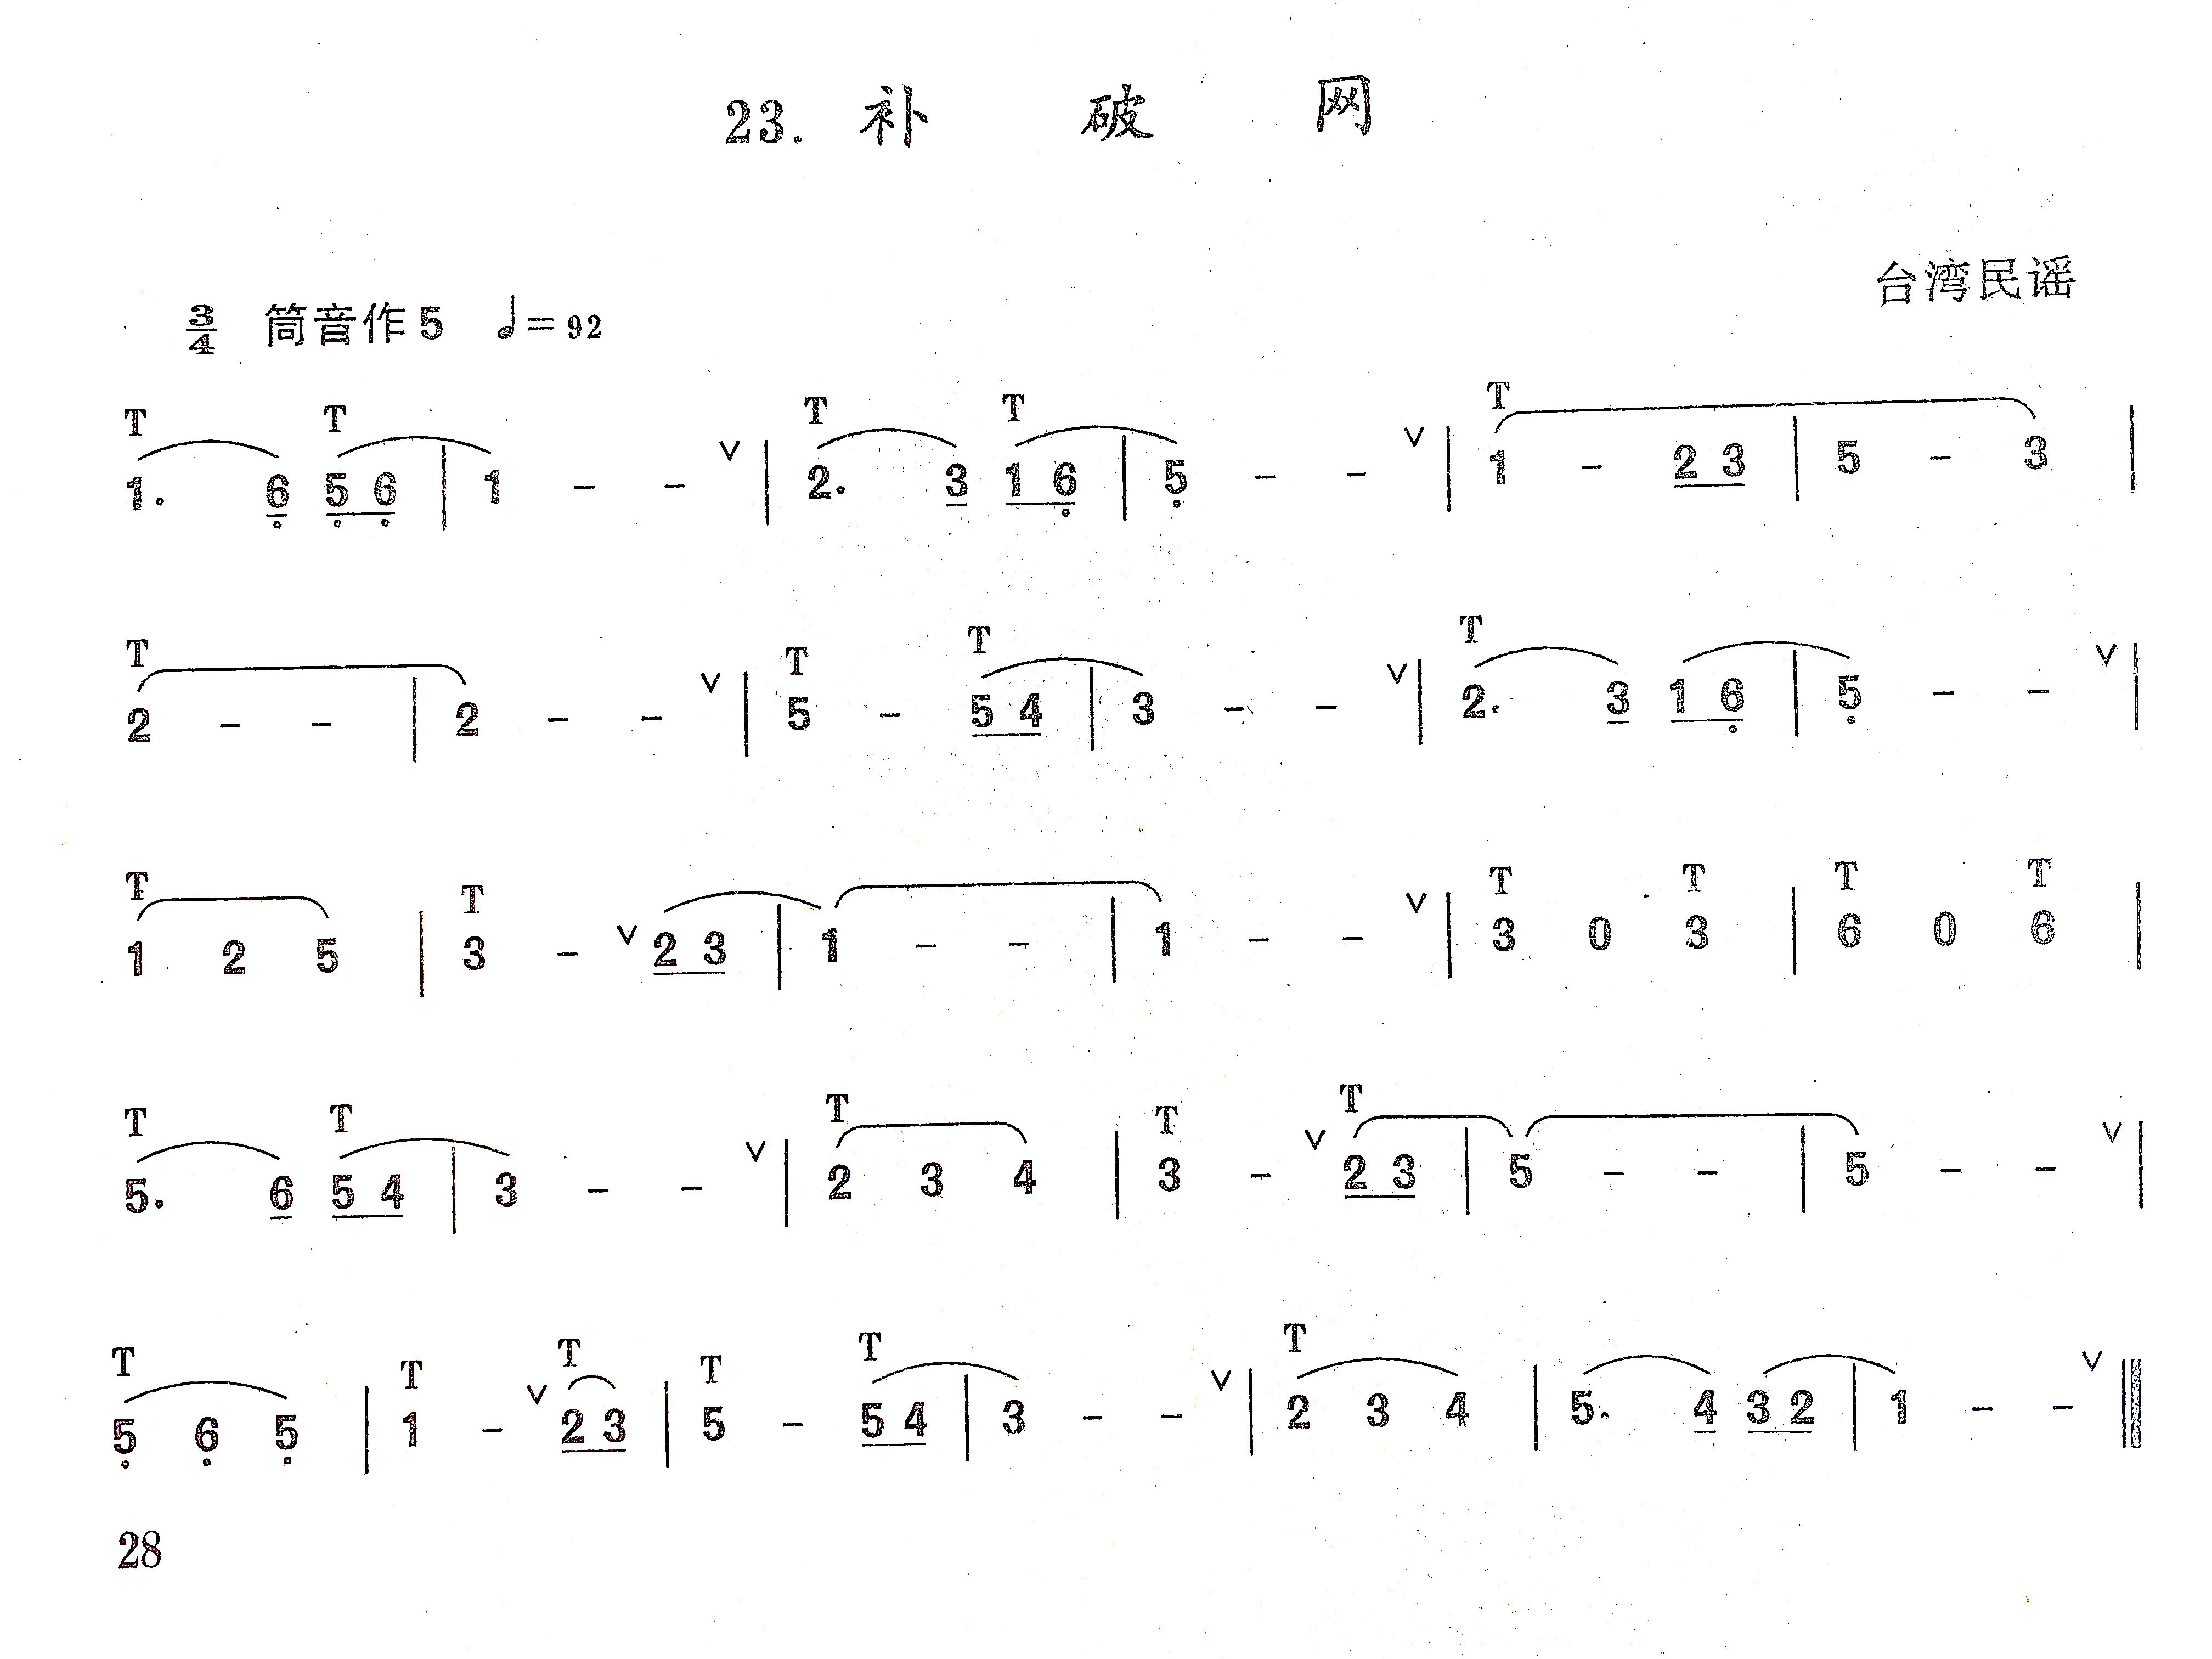
\includegraphics[width=\textwidth]{dongxiao/IMG_0936.jpg}
\section{渔光曲}           
	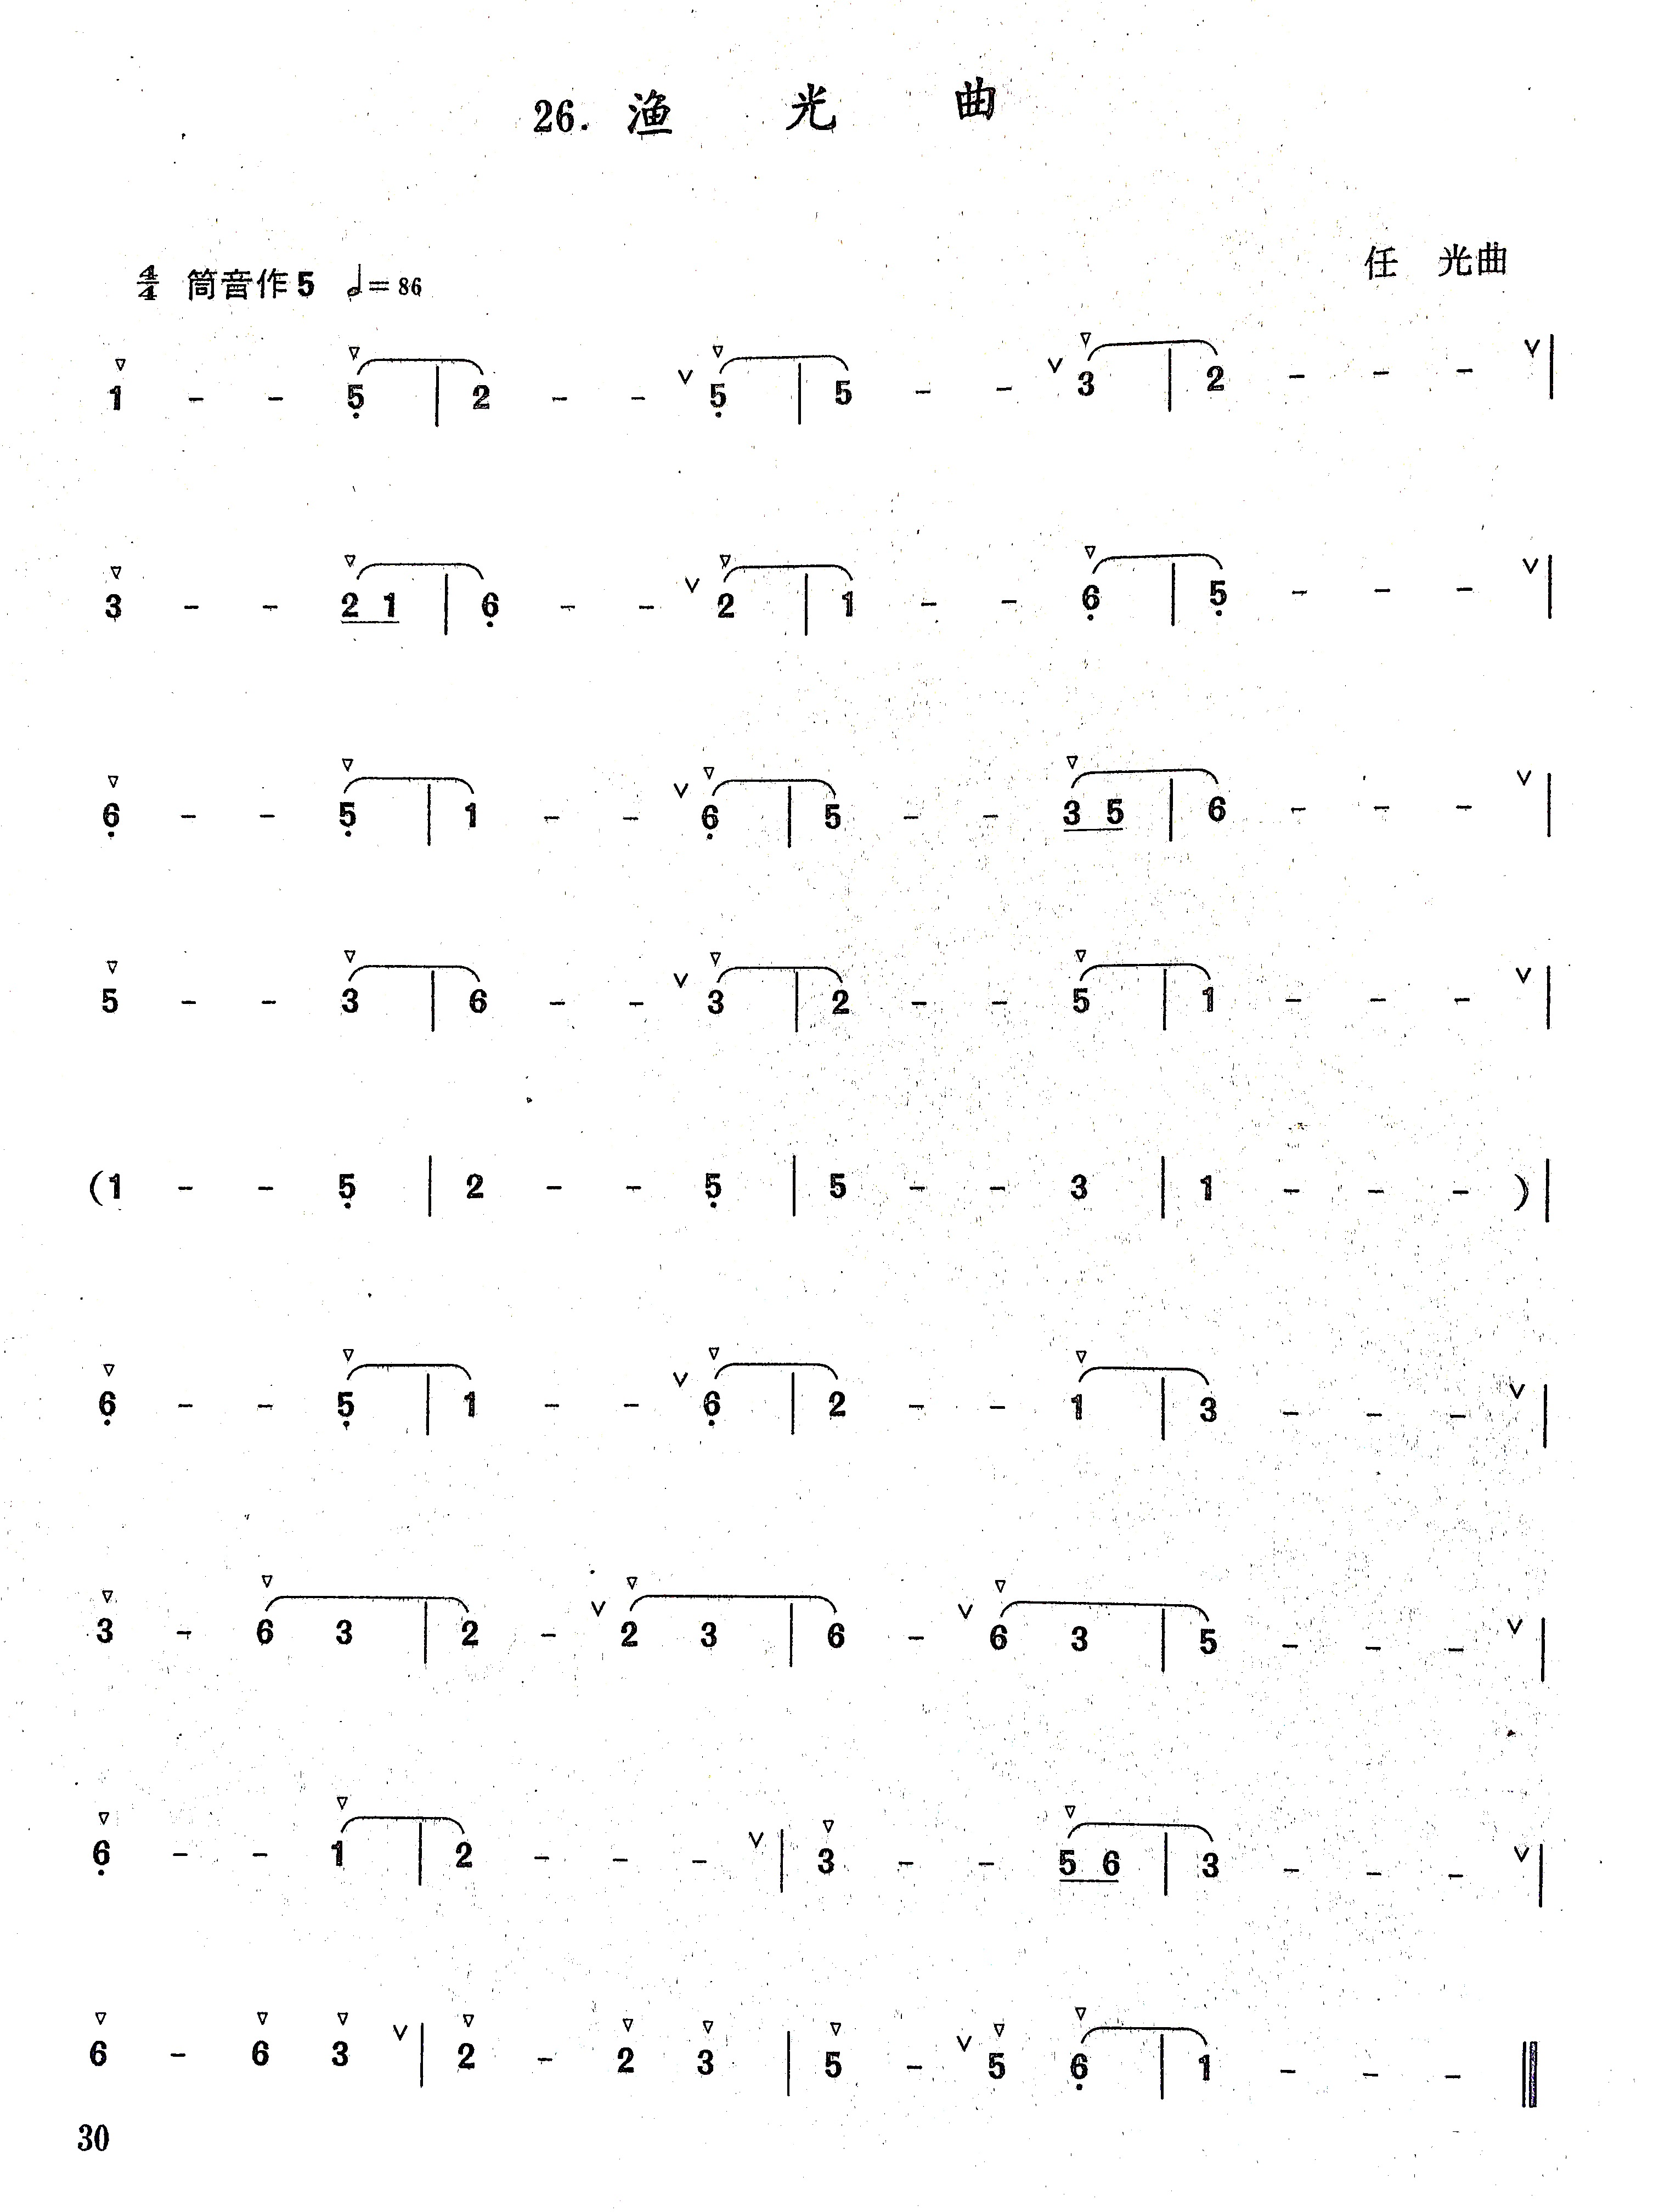
\includegraphics[width=\textwidth]{dongxiao/IMG_0939.jpg}   
\section{秋湖月夜}   
	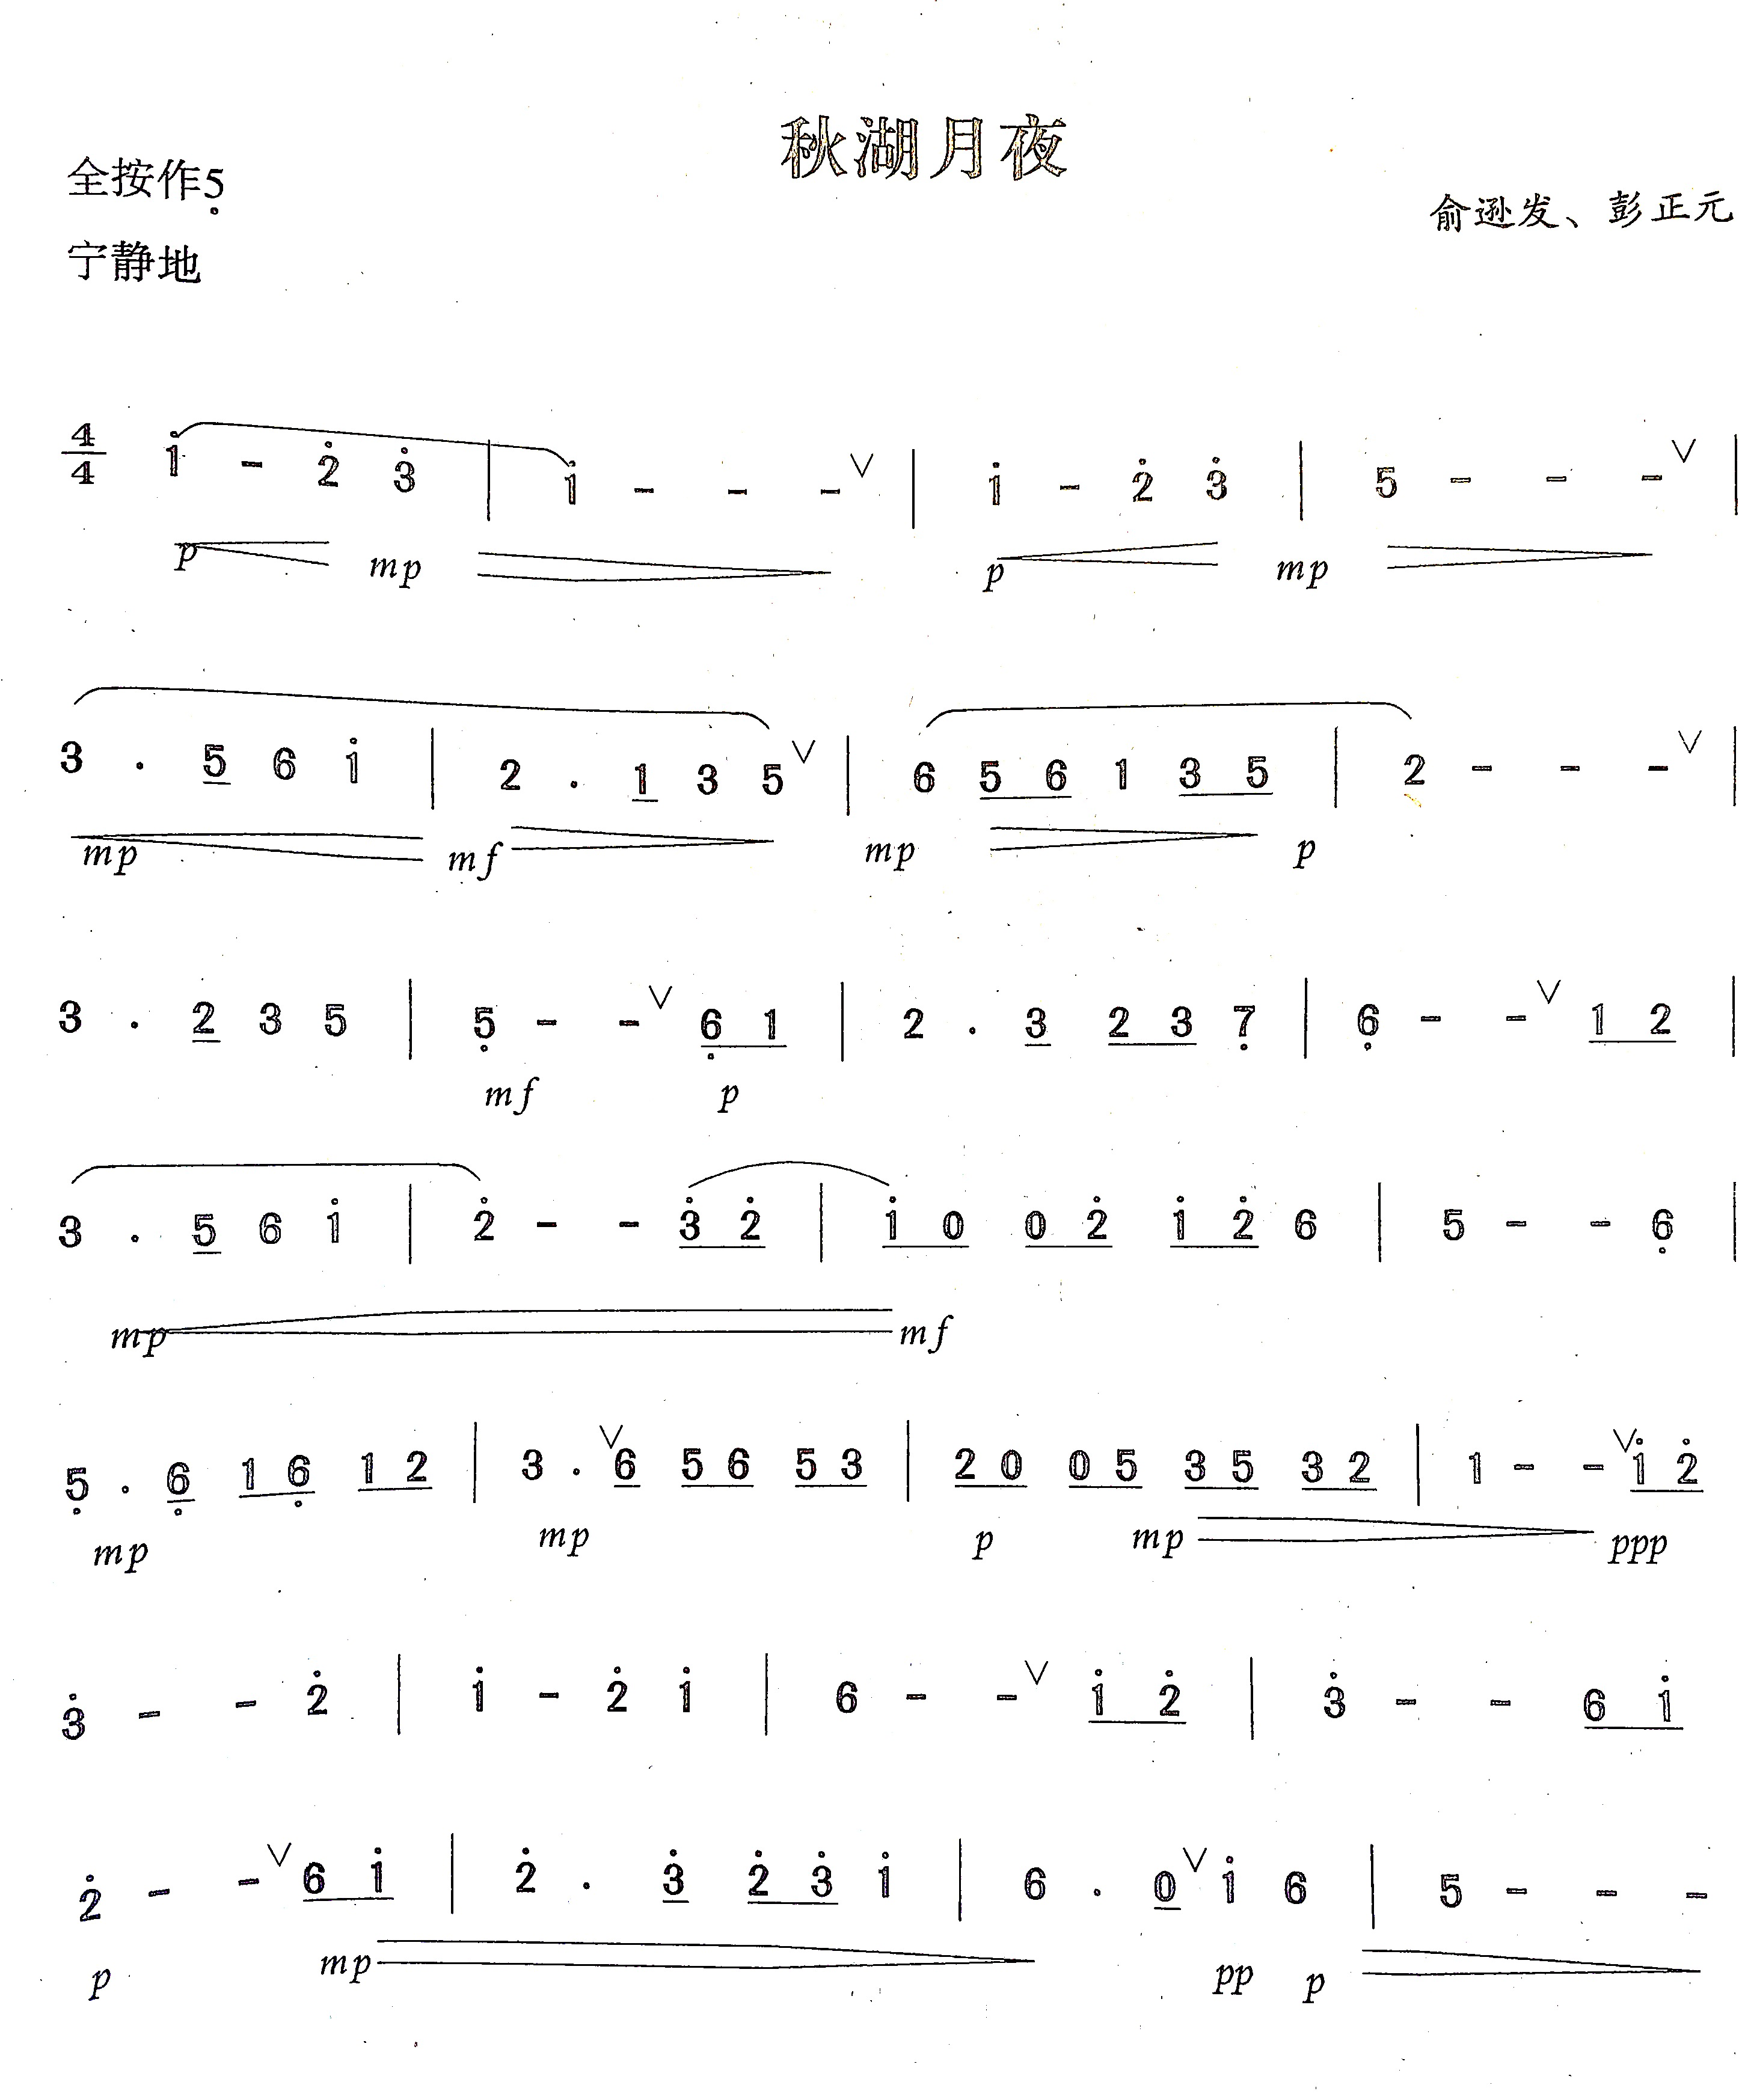
\includegraphics[width=\textwidth]{dongxiao/IMG_0948.jpg}
\section{思归乐}
	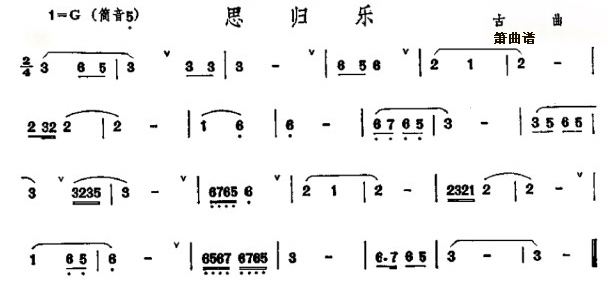
\includegraphics[width=\textwidth]{dongxiao/思归乐.jpg}
\section{秋窗风雨}
    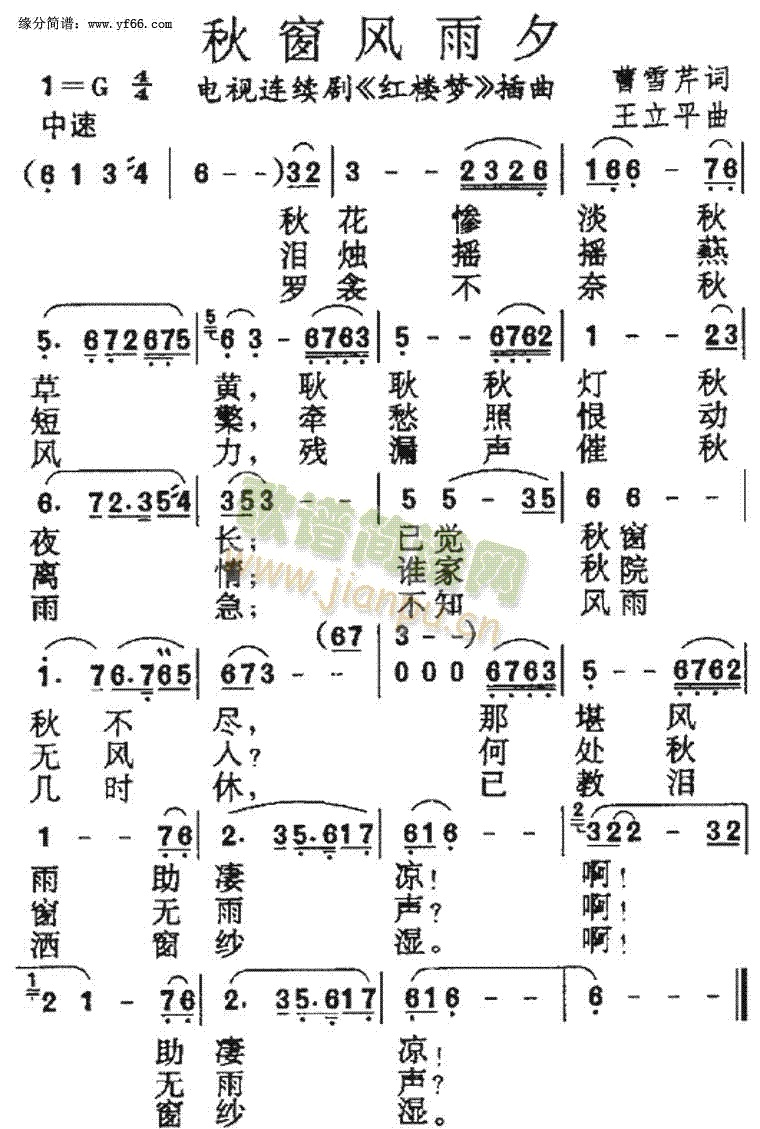
\includegraphics[width=\textwidth]{dongxiao/秋窗风雨.jpg}
\section{红豆曲}
    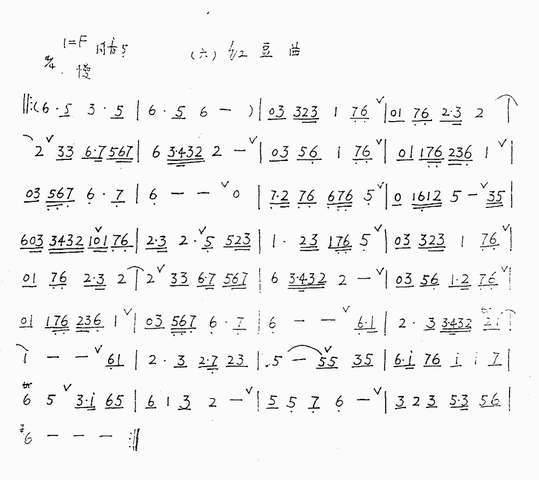
\includegraphics[width=\textwidth]{dongxiao/红豆曲.jpg}

\section{樱花}
	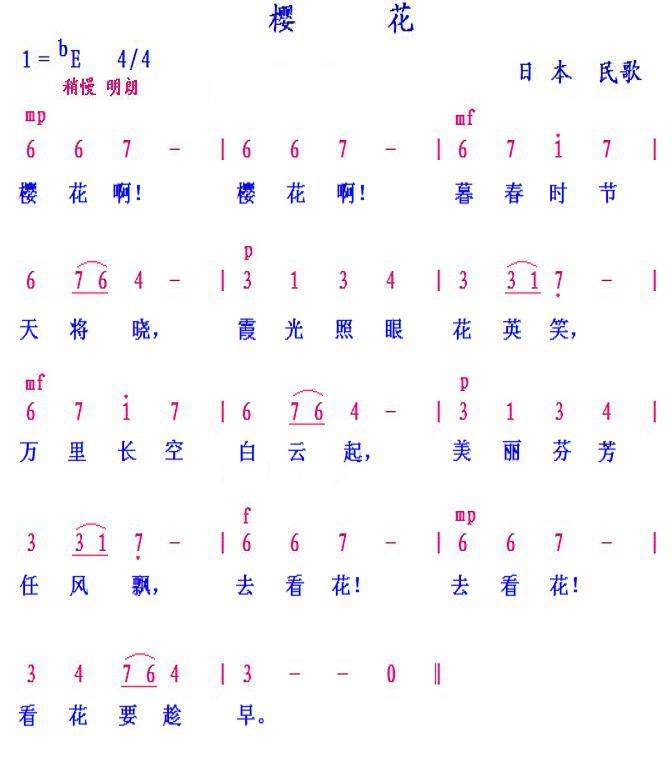
\includegraphics[width=\textwidth]{dongxiao/日本-樱花.jpg}
\section{母亲}
	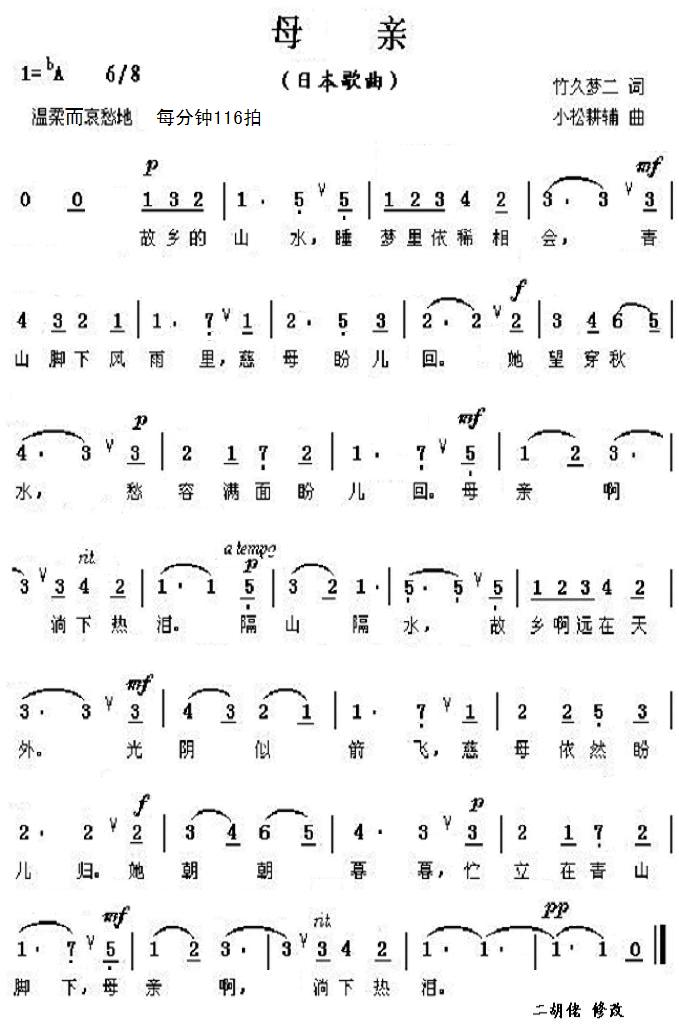
\includegraphics[height=0.9\textheight]{dongxiao/日本-母亲.jpg}


\section{洞箫悠悠}
    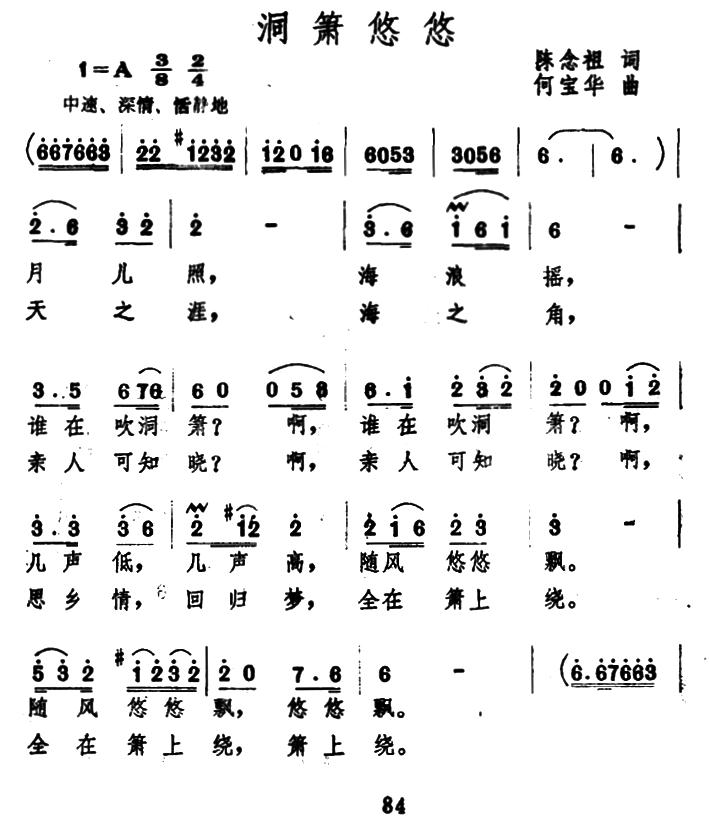
\includegraphics[width=\textwidth]{dongxiao/洞箫悠悠.jpg}
\section{铁血丹心}
    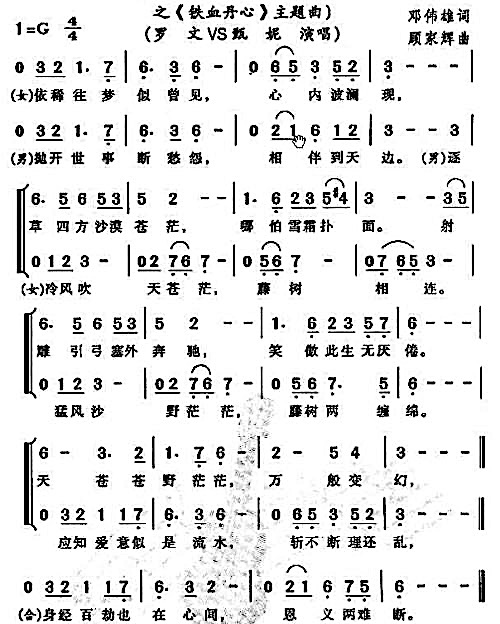
\includegraphics[width=\textwidth]{dongxiao/铁血丹心.jpg}
    
\section{青玉按-元夕}
    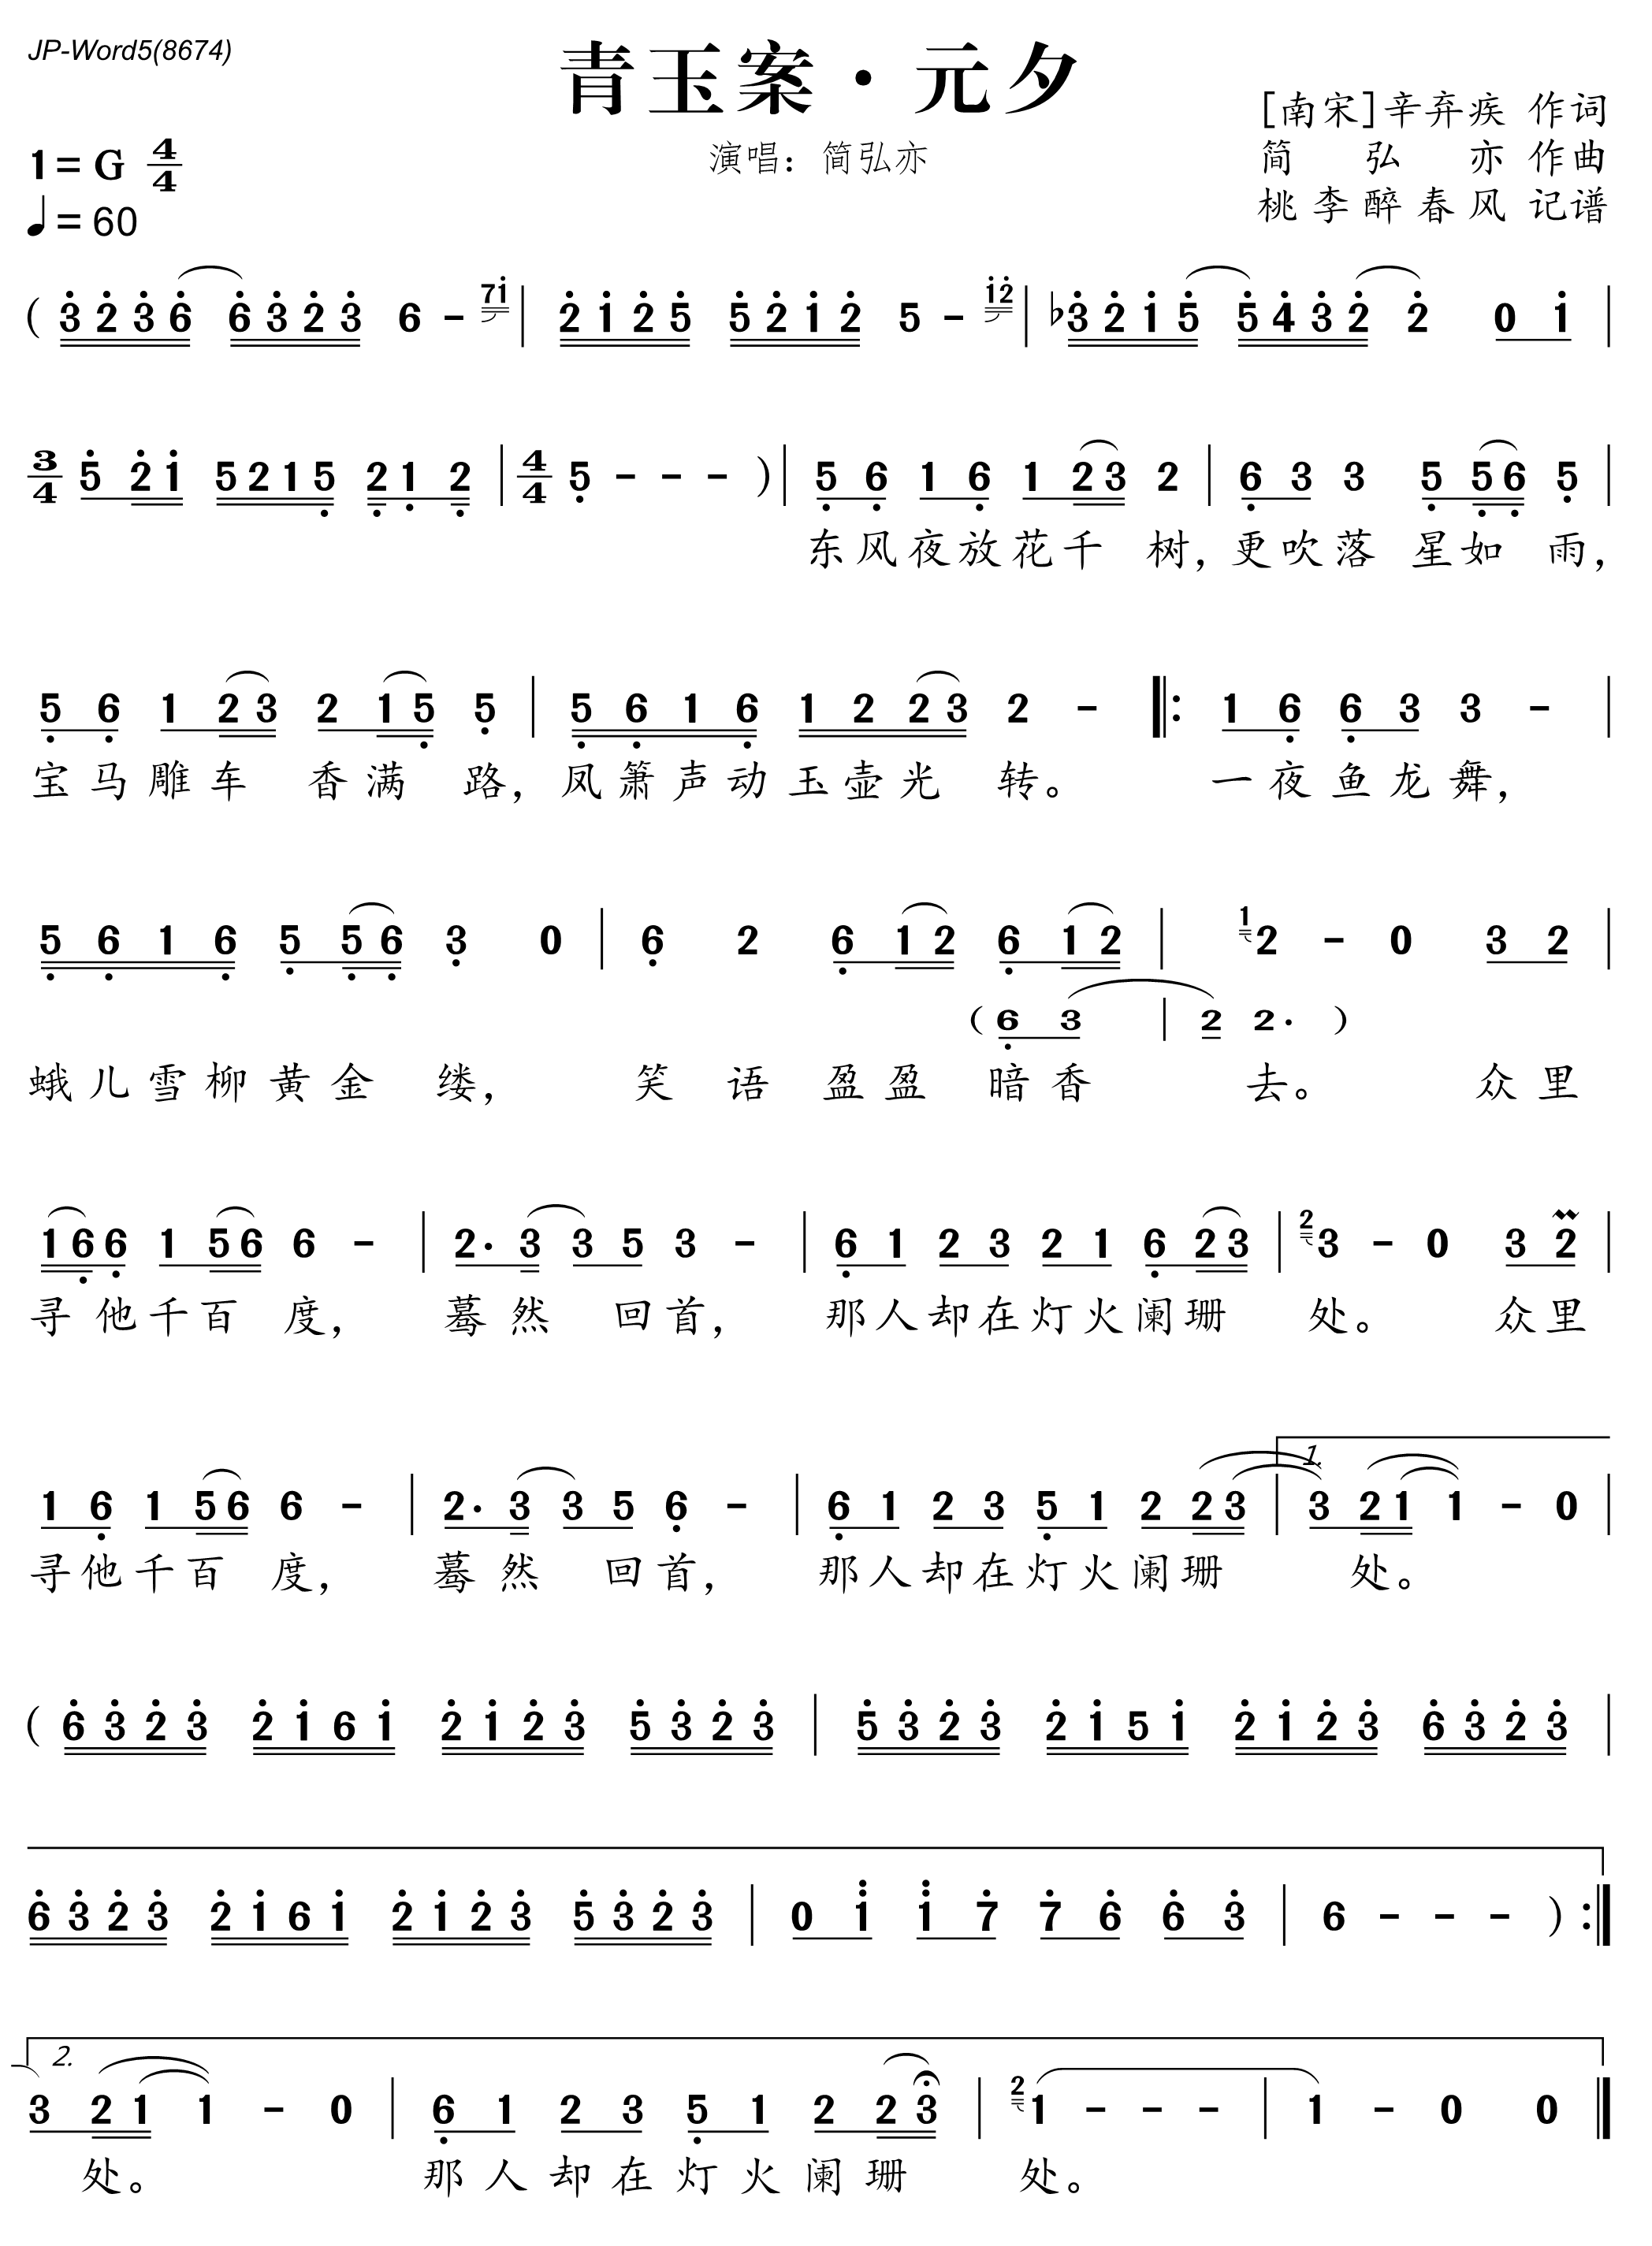
\includegraphics[width=\textwidth]{dongxiao/20200323青玉按.png}
\section{卷珠帘}
    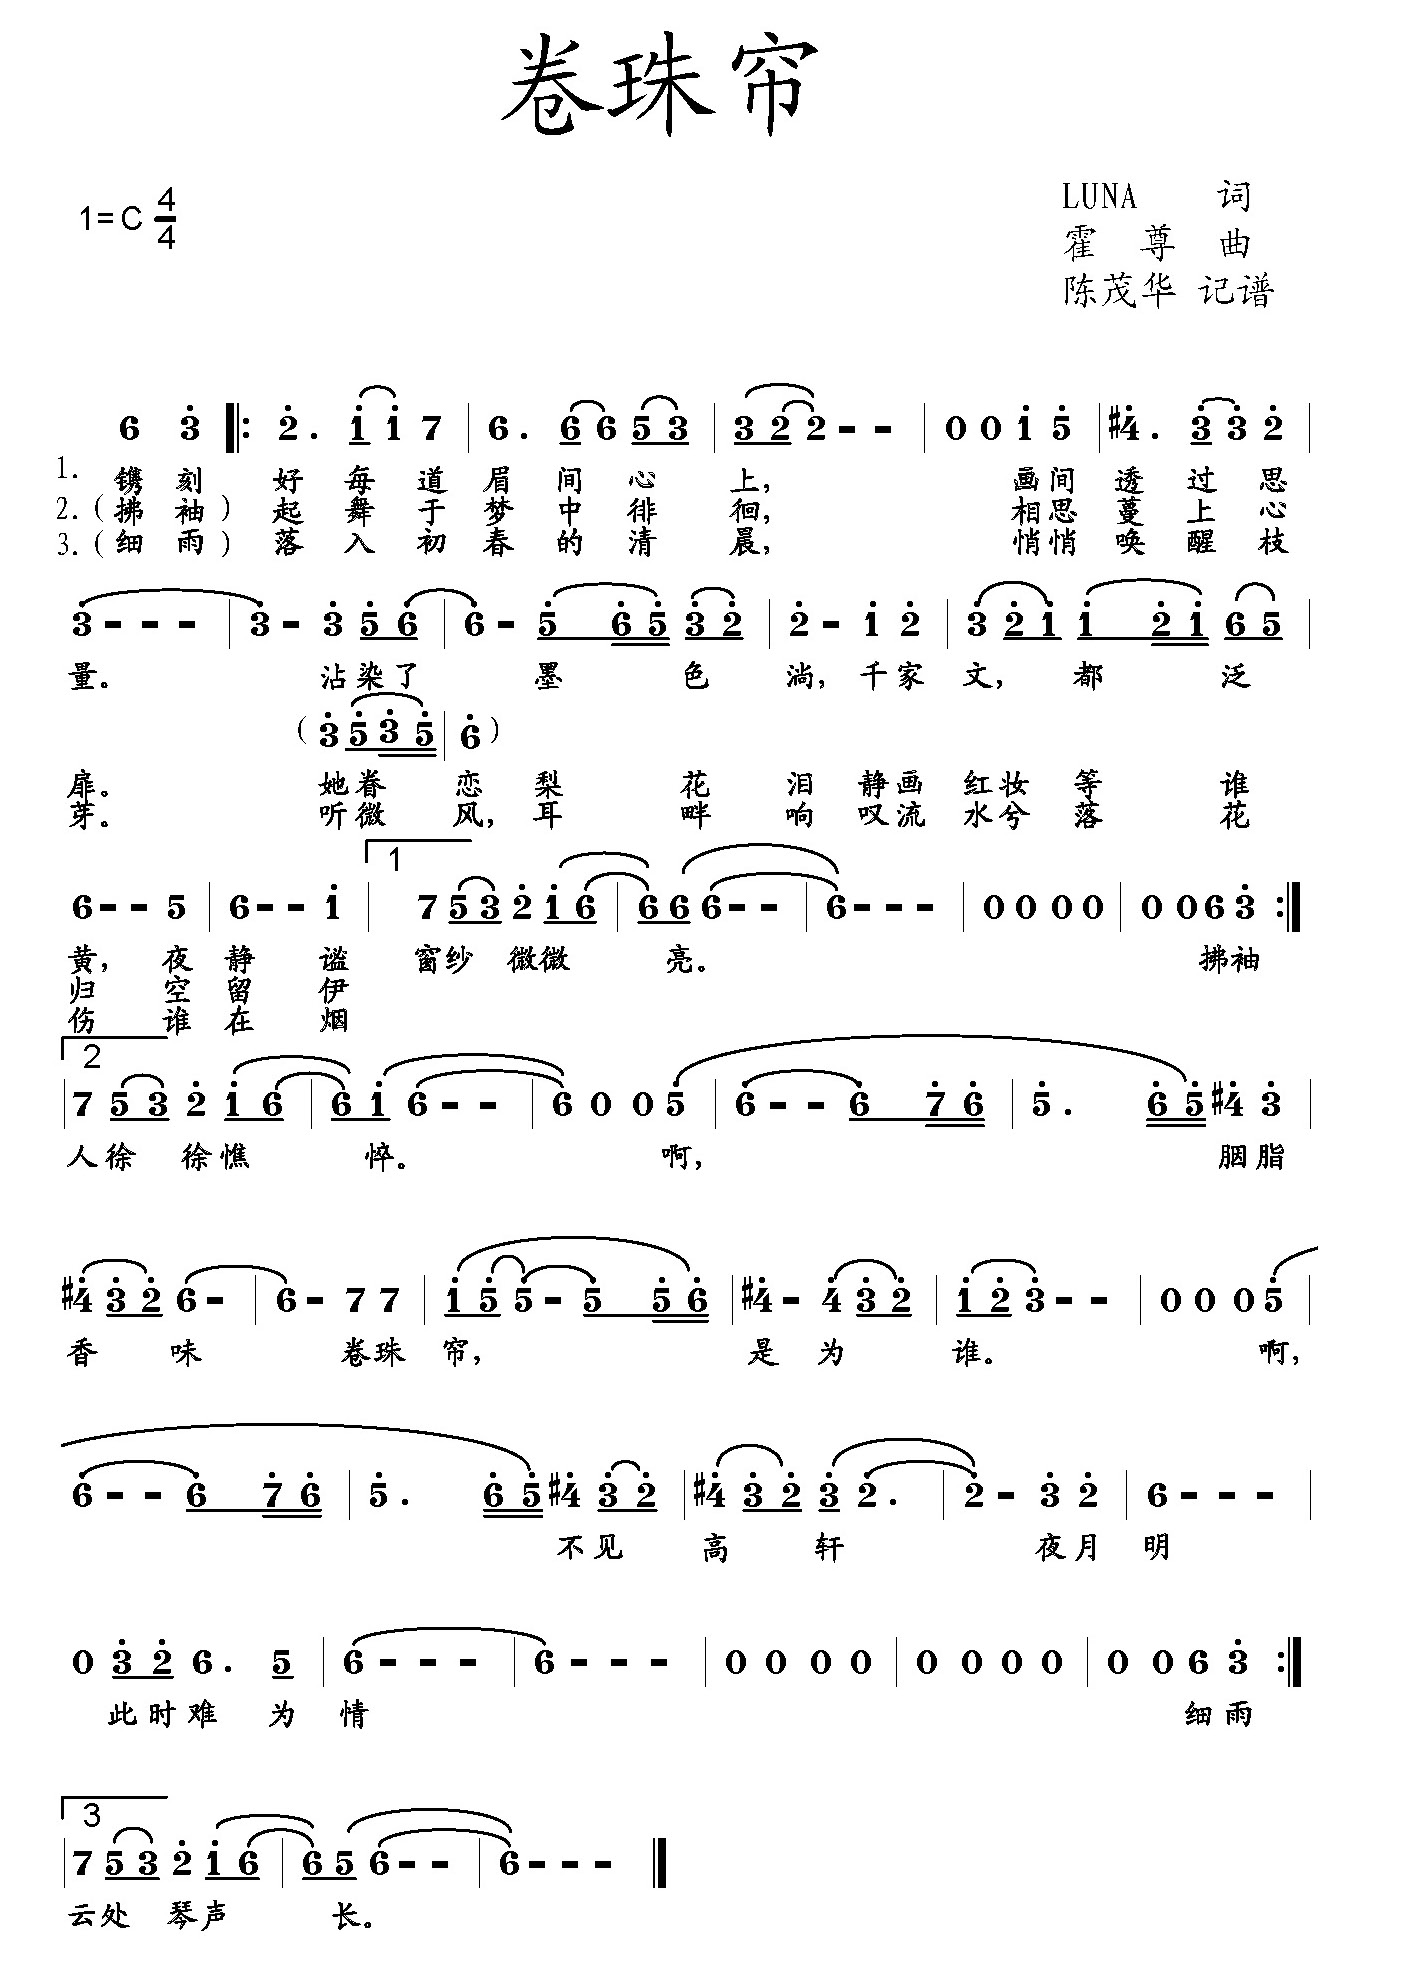
\includegraphics[width=\textwidth]{dongxiao/20200323卷珠帘.jpg}
\section{玉楼春}
    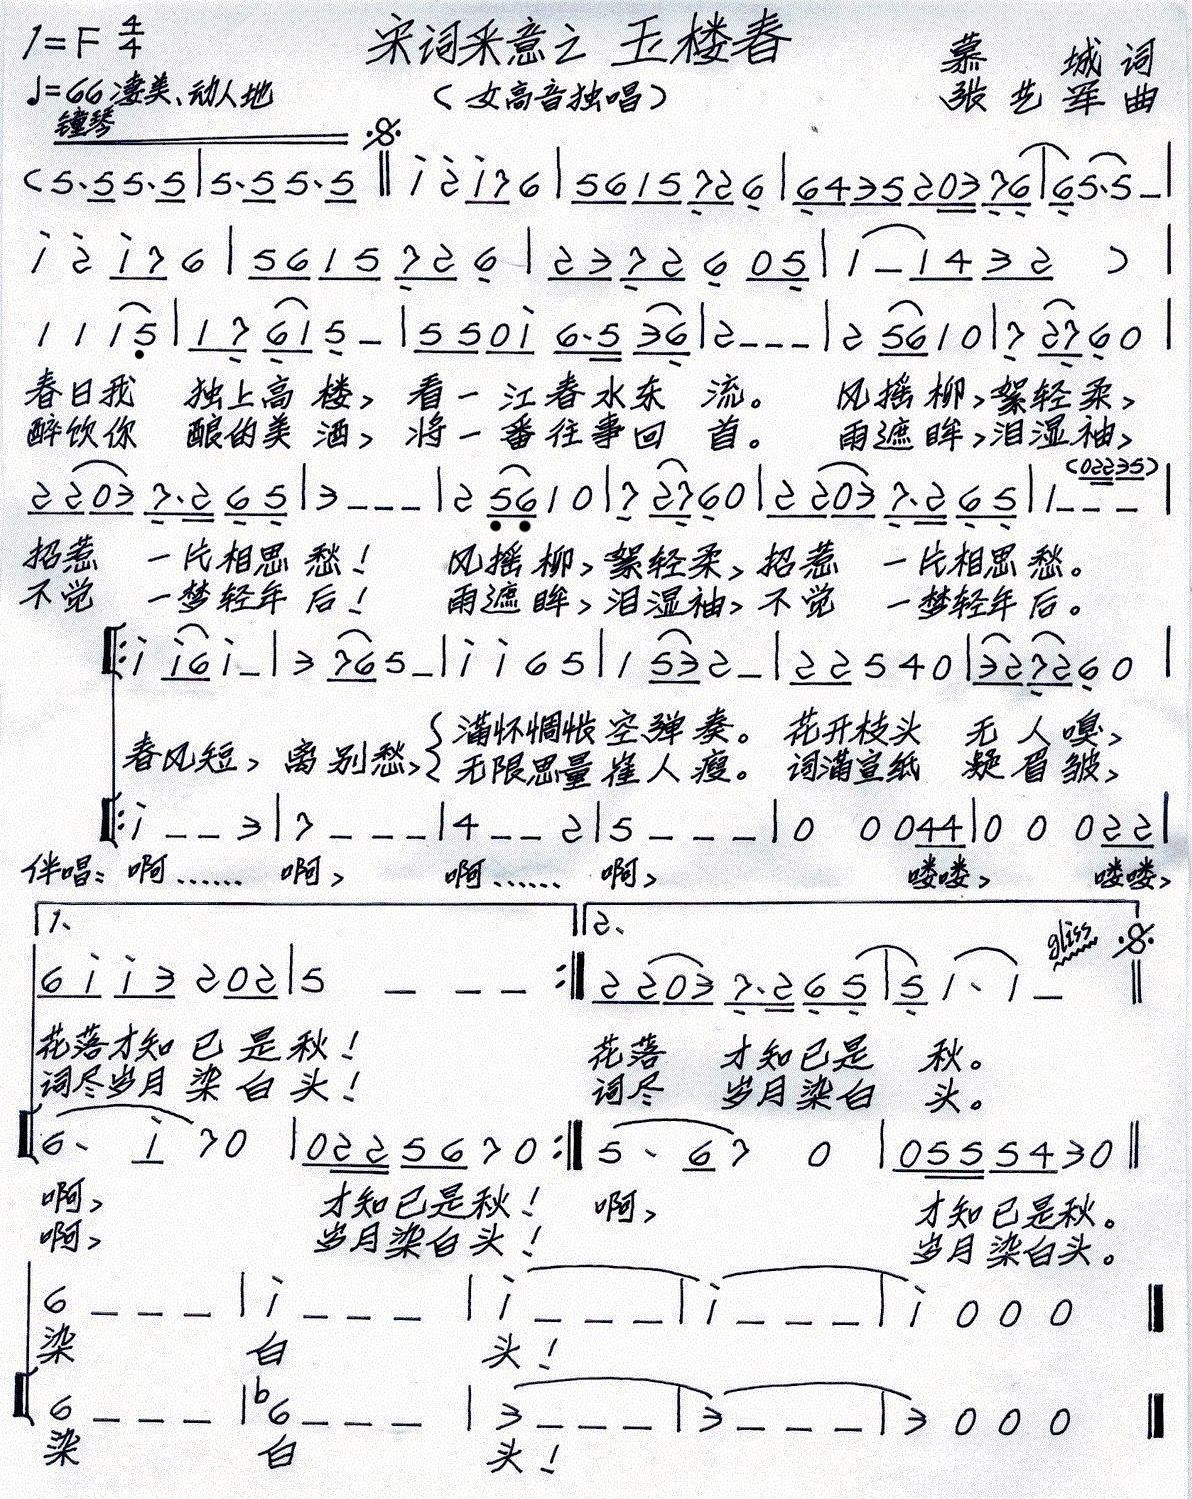
\includegraphics[width=\textwidth]{dongxiao/20200323玉楼春.jpg}
    
\section{风留念}
    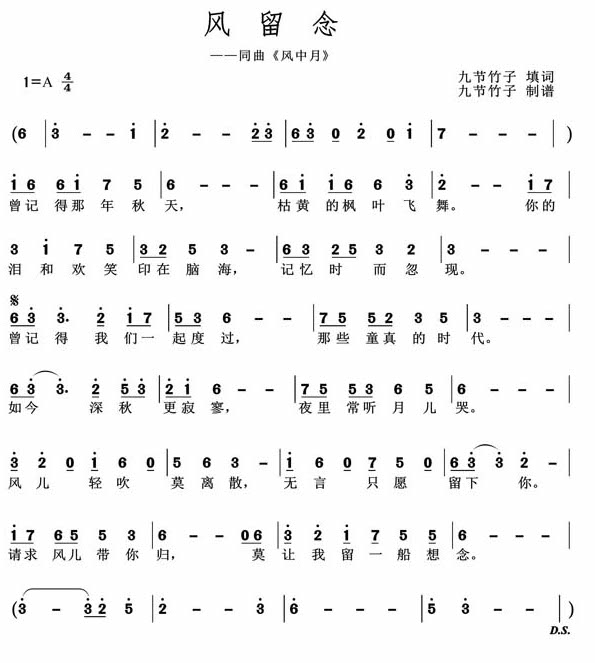
\includegraphics[width=\textwidth]{dongxiao/20200323风留念.jpg}
\section{墨香-长安曲}
    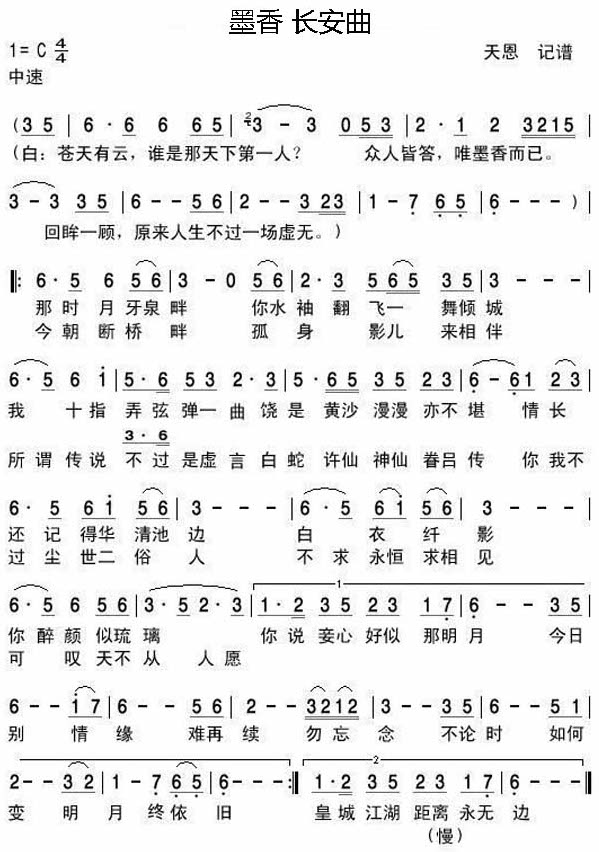
\includegraphics[width=\textwidth]{dongxiao/20200323墨香-长安曲.jpg} 

\chapter{演奏符号}
\section{一}
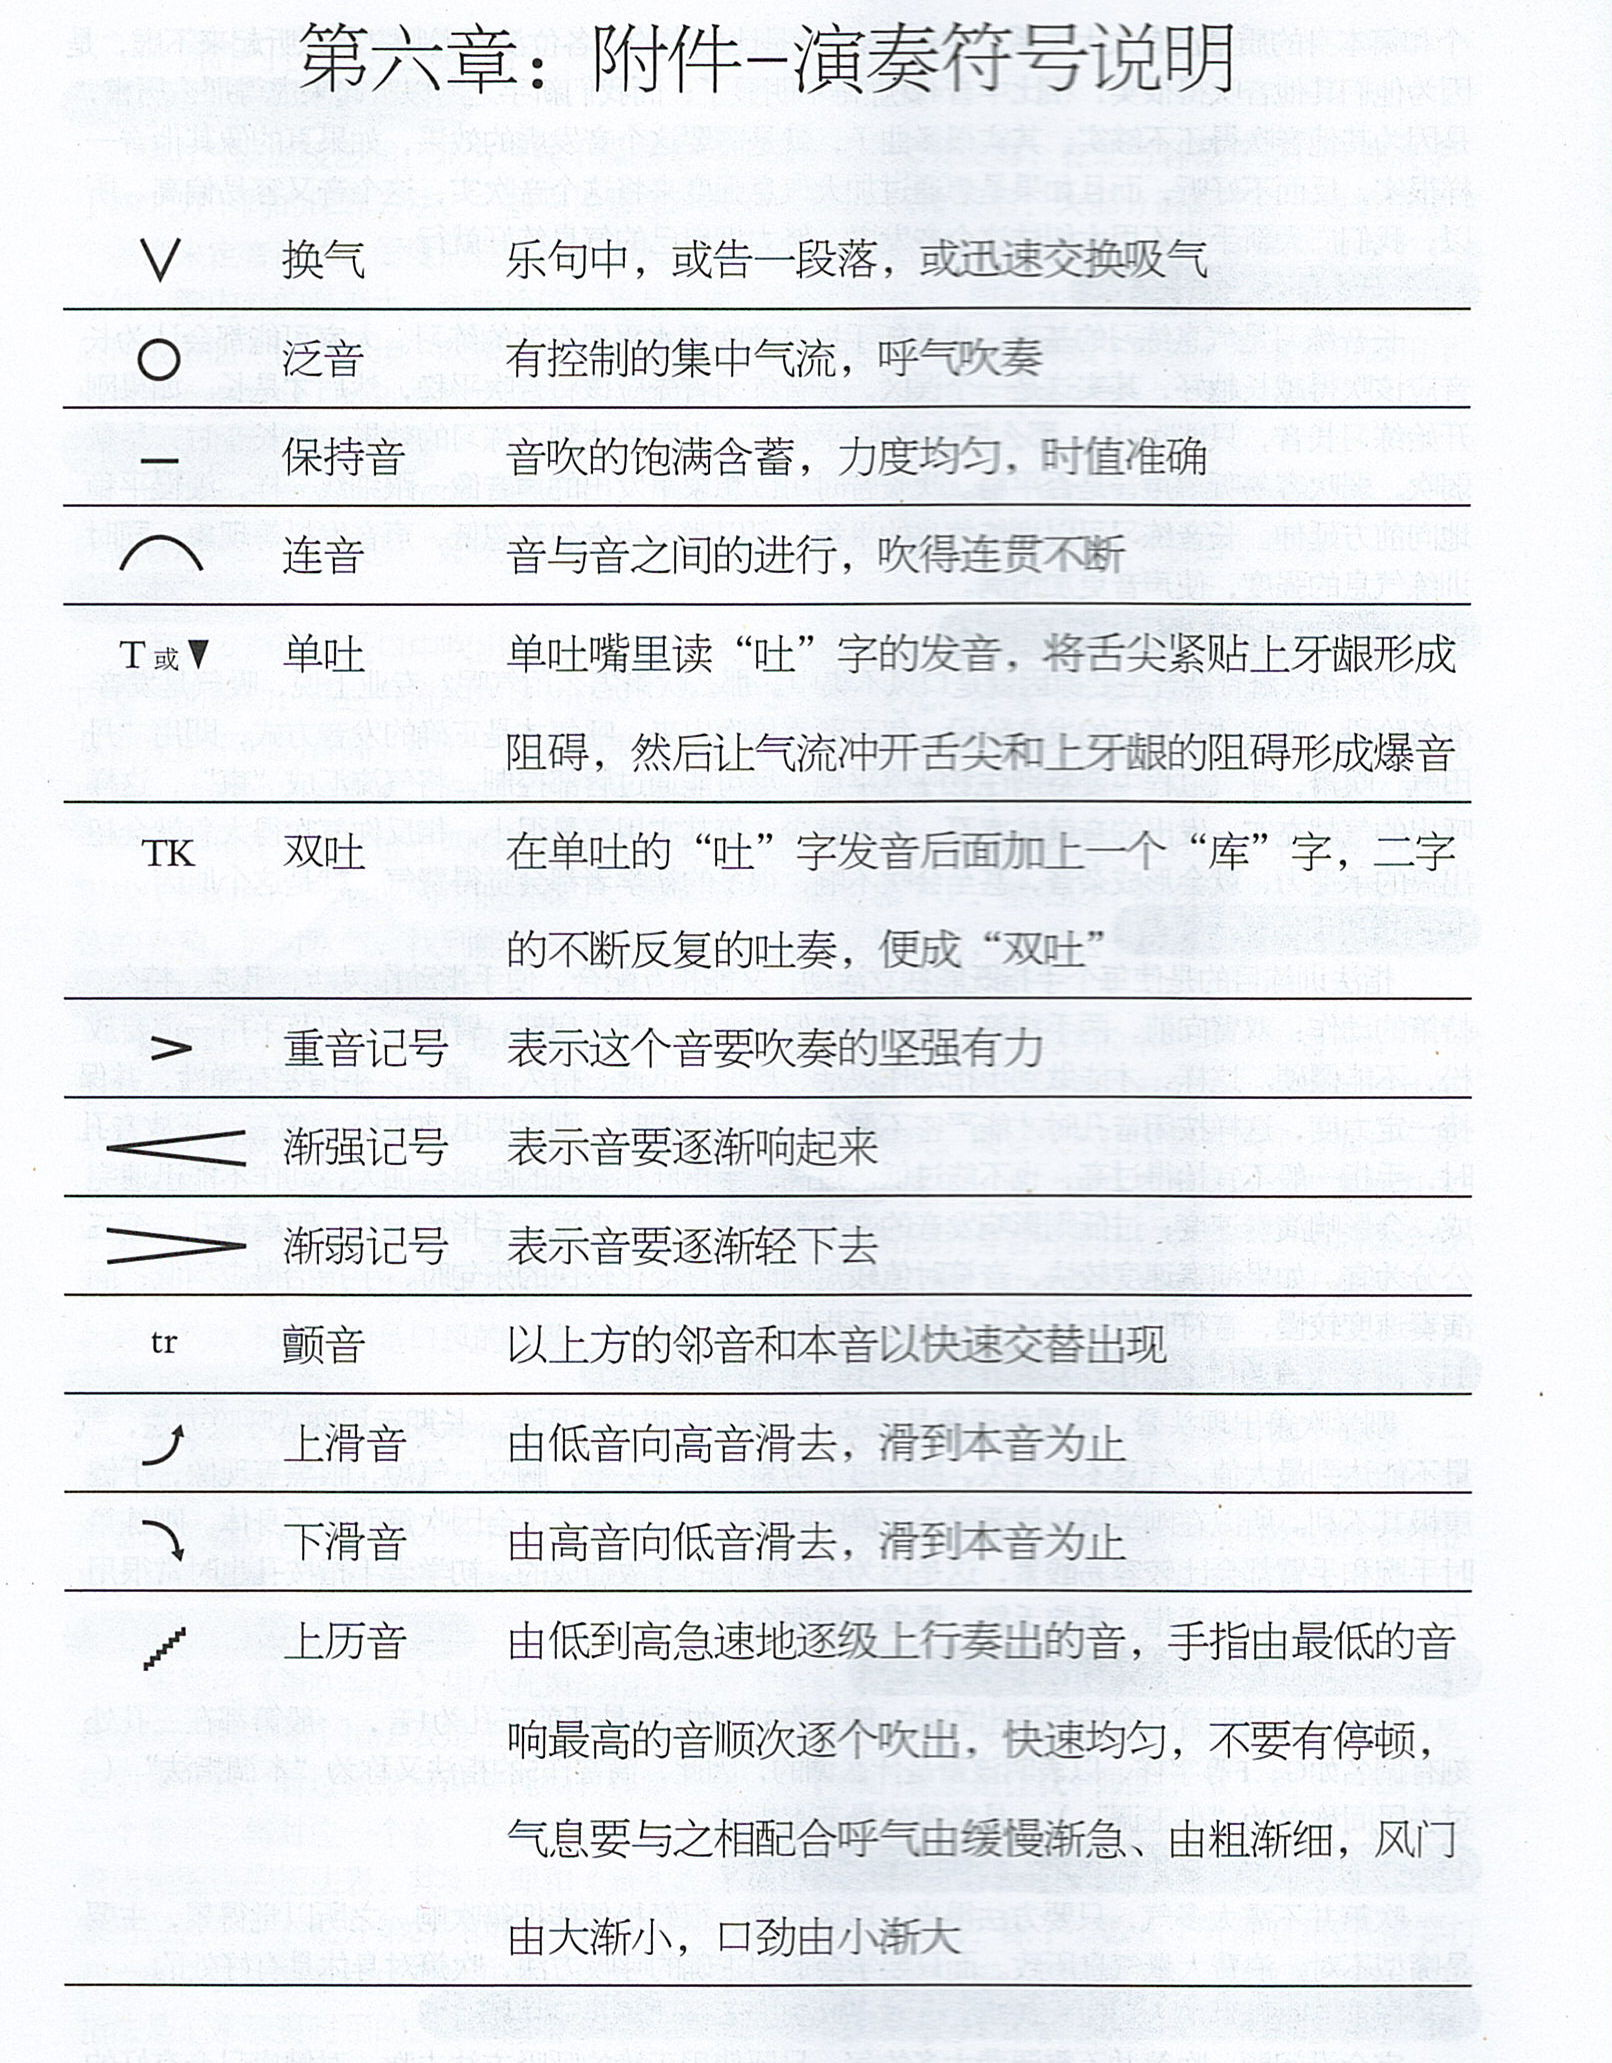
\includegraphics[height=0.8\textheight]{dongxiao/Scan 24.jpeg}
\section{二}
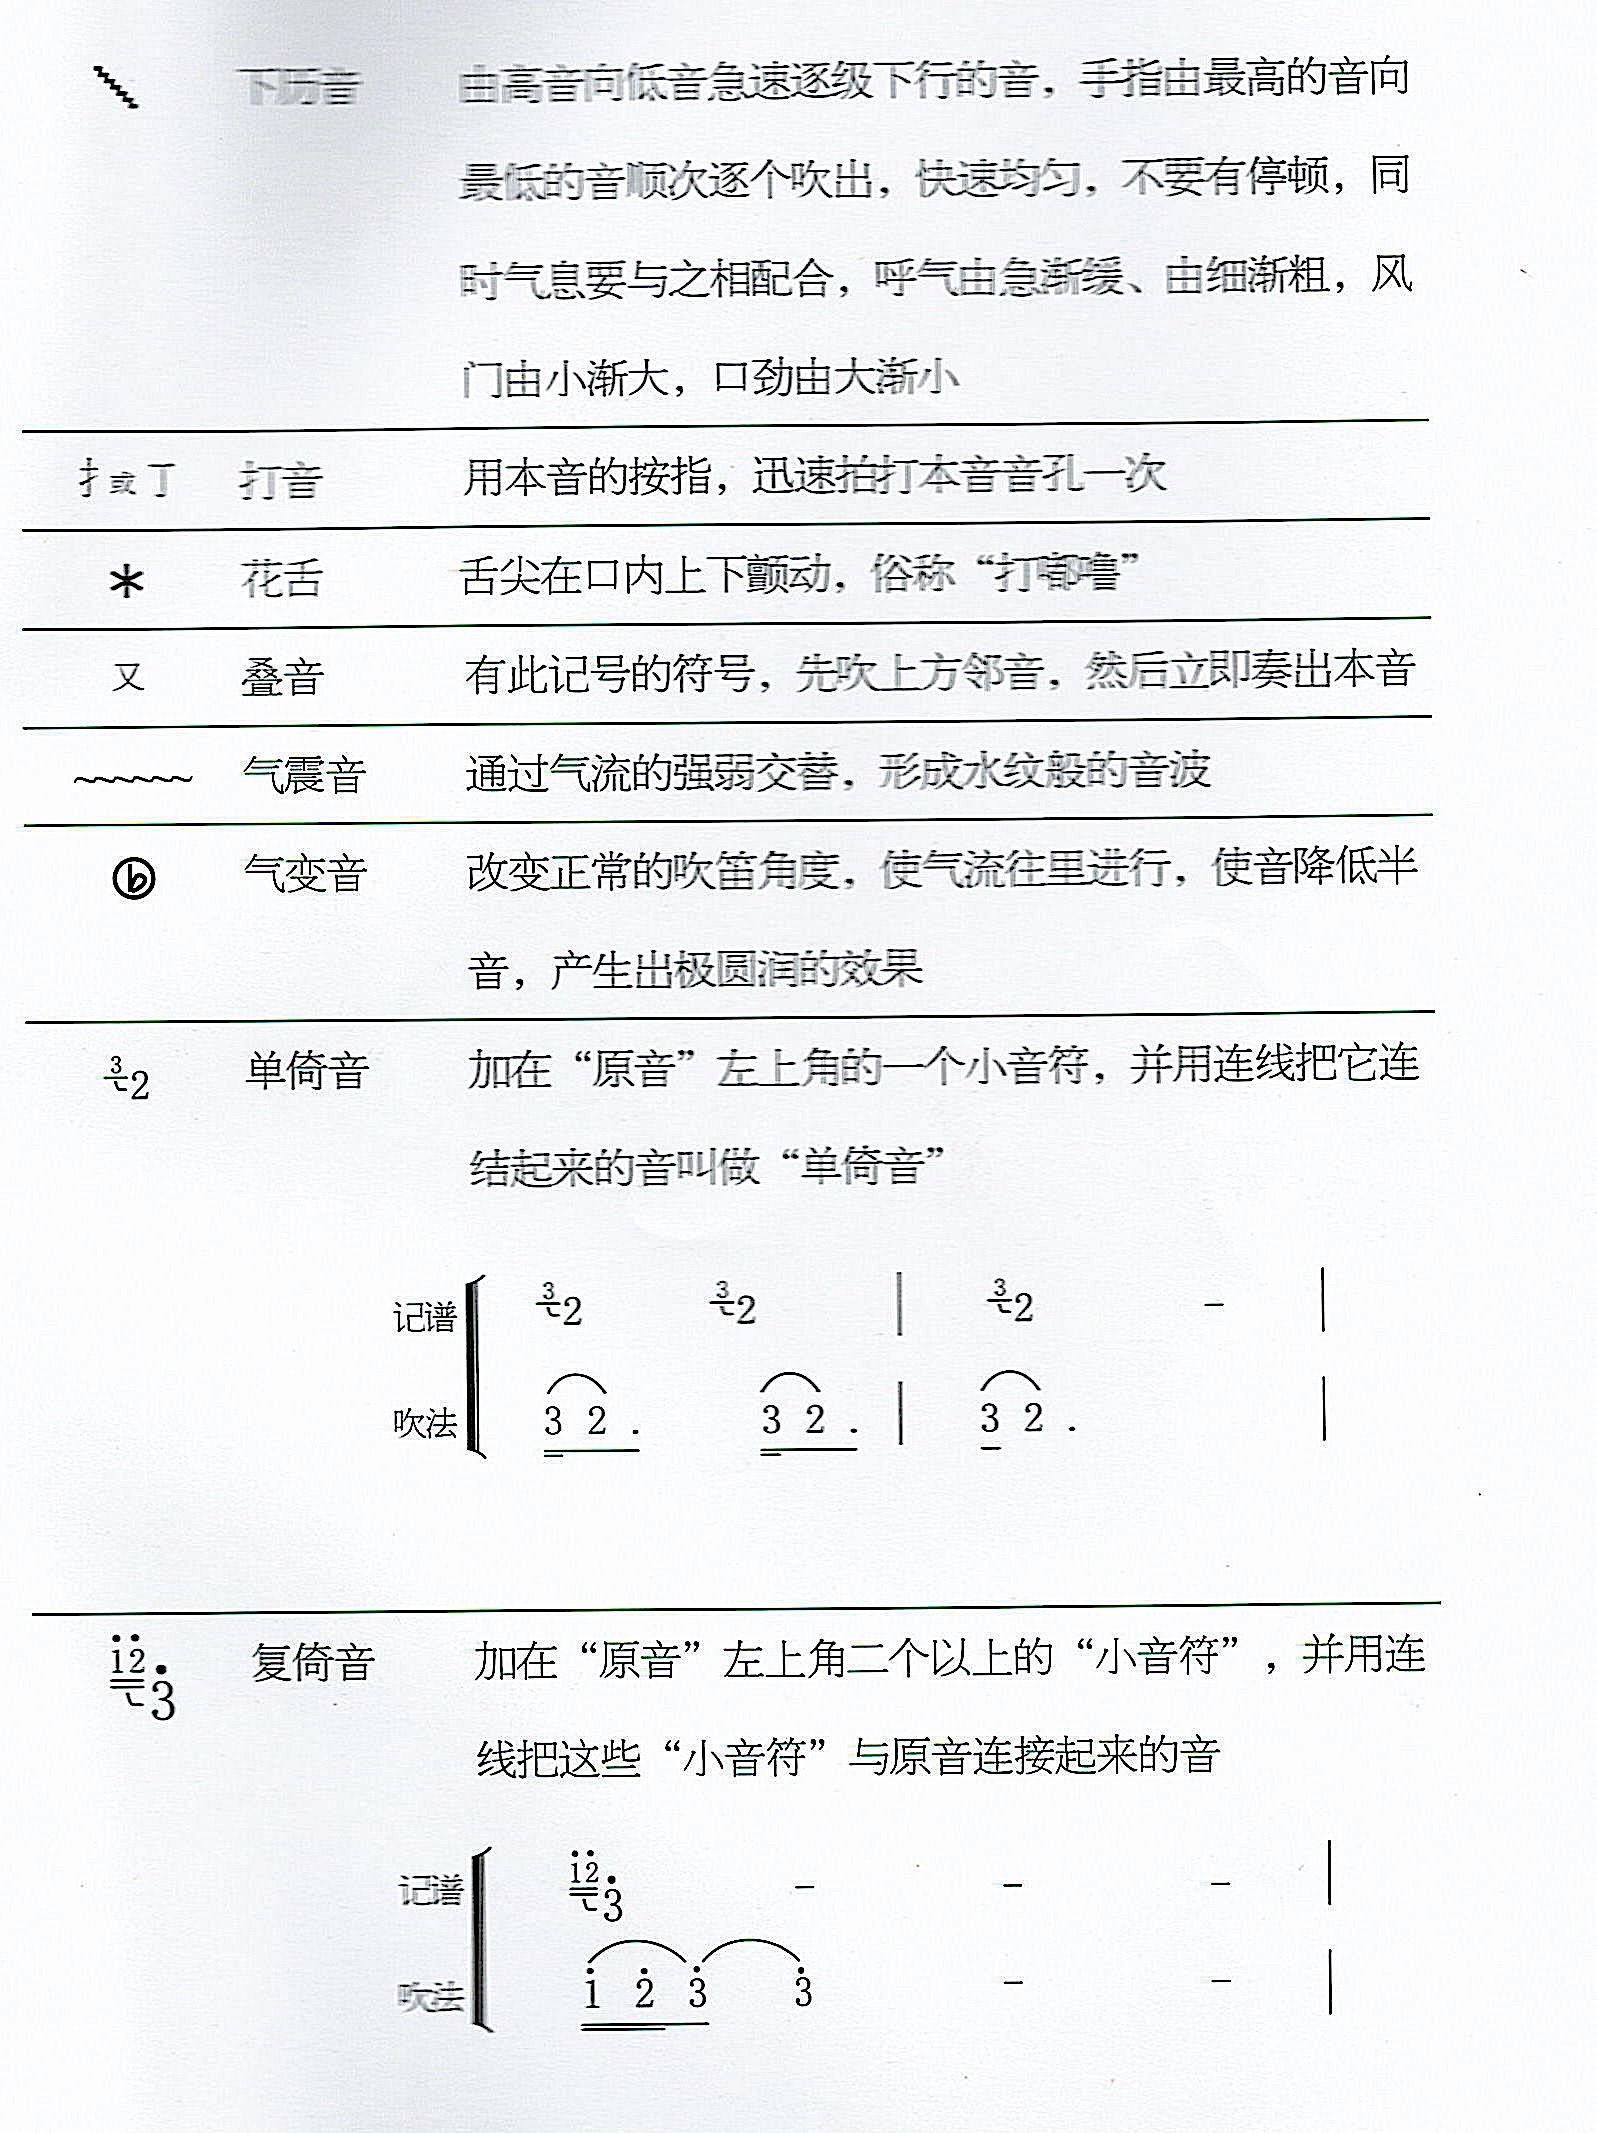
\includegraphics[width=\textwidth]{dongxiao/Scan 25.jpeg}

\end{document}
